\documentclass[twoside]{book}

% Packages required by doxygen
\usepackage{fixltx2e}
\usepackage{calc}
\usepackage{doxygen}
\usepackage[export]{adjustbox} % also loads graphicx
\usepackage{graphicx}
\usepackage[utf8]{inputenc}
\usepackage{makeidx}
\usepackage{multicol}
\usepackage{multirow}
\PassOptionsToPackage{warn}{textcomp}
\usepackage{textcomp}
\usepackage[nointegrals]{wasysym}
\usepackage[table]{xcolor}

% Font selection
\usepackage[T1]{fontenc}
\usepackage[scaled=.90]{helvet}
\usepackage{courier}
\usepackage{amssymb}
\usepackage{sectsty}
\renewcommand{\familydefault}{\sfdefault}
\allsectionsfont{%
  \fontseries{bc}\selectfont%
  \color{darkgray}%
}
\renewcommand{\DoxyLabelFont}{%
  \fontseries{bc}\selectfont%
  \color{darkgray}%
}
\newcommand{\+}{\discretionary{\mbox{\scriptsize$\hookleftarrow$}}{}{}}

% Page & text layout
\usepackage{geometry}
\geometry{%
  a4paper,%
  top=2.5cm,%
  bottom=2.5cm,%
  left=2.5cm,%
  right=2.5cm%
}
\tolerance=750
\hfuzz=15pt
\hbadness=750
\setlength{\emergencystretch}{15pt}
\setlength{\parindent}{0cm}
\setlength{\parskip}{3ex plus 2ex minus 2ex}
\makeatletter
\renewcommand{\paragraph}{%
  \@startsection{paragraph}{4}{0ex}{-1.0ex}{1.0ex}{%
    \normalfont\normalsize\bfseries\SS@parafont%
  }%
}
\renewcommand{\subparagraph}{%
  \@startsection{subparagraph}{5}{0ex}{-1.0ex}{1.0ex}{%
    \normalfont\normalsize\bfseries\SS@subparafont%
  }%
}
\makeatother

% Headers & footers
\usepackage{fancyhdr}
\pagestyle{fancyplain}
\fancyhead[LE]{\fancyplain{}{\bfseries\thepage}}
\fancyhead[CE]{\fancyplain{}{}}
\fancyhead[RE]{\fancyplain{}{\bfseries\leftmark}}
\fancyhead[LO]{\fancyplain{}{\bfseries\rightmark}}
\fancyhead[CO]{\fancyplain{}{}}
\fancyhead[RO]{\fancyplain{}{\bfseries\thepage}}
\fancyfoot[LE]{\fancyplain{}{}}
\fancyfoot[CE]{\fancyplain{}{}}
\fancyfoot[RE]{\fancyplain{}{\bfseries\scriptsize Generated by Doxygen }}
\fancyfoot[LO]{\fancyplain{}{\bfseries\scriptsize Generated by Doxygen }}
\fancyfoot[CO]{\fancyplain{}{}}
\fancyfoot[RO]{\fancyplain{}{}}
\renewcommand{\footrulewidth}{0.4pt}
\renewcommand{\chaptermark}[1]{%
  \markboth{#1}{}%
}
\renewcommand{\sectionmark}[1]{%
  \markright{\thesection\ #1}%
}

% Indices & bibliography
\usepackage{natbib}
\usepackage[titles]{tocloft}
\setcounter{tocdepth}{3}
\setcounter{secnumdepth}{5}
\makeindex

% Hyperlinks (required, but should be loaded last)
\usepackage{ifpdf}
\ifpdf
  \usepackage[pdftex,pagebackref=true]{hyperref}
\else
  \usepackage[ps2pdf,pagebackref=true]{hyperref}
\fi
\hypersetup{%
  colorlinks=true,%
  linkcolor=blue,%
  citecolor=blue,%
  unicode%
}

% Custom commands
\newcommand{\clearemptydoublepage}{%
  \newpage{\pagestyle{empty}\cleardoublepage}%
}

\usepackage{caption}
\captionsetup{labelsep=space,justification=centering,font={bf},singlelinecheck=off,skip=4pt,position=top}

%===== C O N T E N T S =====

\begin{document}

% Titlepage & ToC
\hypersetup{pageanchor=false,
             bookmarksnumbered=true,
             pdfencoding=unicode
            }
\pagenumbering{alph}
\begin{titlepage}
\vspace*{7cm}
\begin{center}%
{\Large Project Mary Poppins }\\
\vspace*{1cm}
{\large Generated by Doxygen 1.8.13}\\
\end{center}
\end{titlepage}
\clearemptydoublepage
\pagenumbering{roman}
\tableofcontents
\clearemptydoublepage
\pagenumbering{arabic}
\hypersetup{pageanchor=true}

%--- Begin generated contents ---
\chapter{Namespace Index}
\section{Namespace List}
Here is a list of all documented namespaces with brief descriptions\+:\begin{DoxyCompactList}
\item\contentsline{section}{\hyperlink{namespacecleanup}{cleanup} \\*Namespace for Cleanup Implementation }{\pageref{namespacecleanup}}{}
\end{DoxyCompactList}

\chapter{Hierarchical Index}
\section{Class Hierarchy}
This inheritance list is sorted roughly, but not completely, alphabetically\+:\begin{DoxyCompactList}
\item \contentsline{section}{augment\+\_\+args}{\pageref{structaugment__args}}{}
\item \contentsline{section}{box}{\pageref{structbox}}{}
\item \contentsline{section}{box\+\_\+label}{\pageref{structbox__label}}{}
\item \contentsline{section}{cleanup\+:\+:Controller}{\pageref{classcleanup_1_1_controller}}{}
\item \contentsline{section}{data}{\pageref{structdata}}{}
\item \contentsline{section}{dbox}{\pageref{structdbox}}{}
\item \contentsline{section}{detection}{\pageref{structdetection}}{}
\item \contentsline{section}{image}{\pageref{structimage}}{}
\item \contentsline{section}{kvp}{\pageref{structkvp}}{}
\item \contentsline{section}{layer}{\pageref{structlayer}}{}
\item \contentsline{section}{list}{\pageref{structlist}}{}
\item \contentsline{section}{load\+\_\+args}{\pageref{structload__args}}{}
\item \contentsline{section}{matrix}{\pageref{structmatrix}}{}
\item \contentsline{section}{metadata}{\pageref{structmetadata}}{}
\item \contentsline{section}{cleanup\+:\+:Navigation}{\pageref{classcleanup_1_1_navigation}}{}
\item \contentsline{section}{network}{\pageref{structnetwork}}{}
\item \contentsline{section}{node}{\pageref{structnode}}{}
\item Panel\begin{DoxyCompactList}
\item \contentsline{section}{cleanup\+:\+:User\+Panel}{\pageref{classcleanup_1_1_user_panel}}{}
\end{DoxyCompactList}
\item \contentsline{section}{cleanup\+:\+:Perception}{\pageref{classcleanup_1_1_perception}}{}
\item \contentsline{section}{stbi\+\_\+io\+\_\+callbacks}{\pageref{structstbi__io__callbacks}}{}
\item \contentsline{section}{tree}{\pageref{structtree}}{}
\item \contentsline{section}{update\+\_\+args}{\pageref{structupdate__args}}{}
\end{DoxyCompactList}

\chapter{Class Index}
\section{Class List}
Here are the classes, structs, unions and interfaces with brief descriptions\+:\begin{DoxyCompactList}
\item\contentsline{section}{\hyperlink{structaugment__args}{augment\+\_\+args} }{\pageref{structaugment__args}}{}
\item\contentsline{section}{\hyperlink{structbox}{box} }{\pageref{structbox}}{}
\item\contentsline{section}{\hyperlink{structbox__label}{box\+\_\+label} }{\pageref{structbox__label}}{}
\item\contentsline{section}{\hyperlink{classcleanup_1_1_controller}{cleanup\+::\+Controller} \\*Implementation for a \hyperlink{classcleanup_1_1_controller}{Controller} in R\+OS to command a turtlebot rover }{\pageref{classcleanup_1_1_controller}}{}
\item\contentsline{section}{\hyperlink{structdata}{data} }{\pageref{structdata}}{}
\item\contentsline{section}{\hyperlink{structdbox}{dbox} }{\pageref{structdbox}}{}
\item\contentsline{section}{\hyperlink{structdetection}{detection} }{\pageref{structdetection}}{}
\item\contentsline{section}{\hyperlink{structimage}{image} }{\pageref{structimage}}{}
\item\contentsline{section}{\hyperlink{structkvp}{kvp} }{\pageref{structkvp}}{}
\item\contentsline{section}{\hyperlink{structlayer}{layer} }{\pageref{structlayer}}{}
\item\contentsline{section}{\hyperlink{structlist}{list} }{\pageref{structlist}}{}
\item\contentsline{section}{\hyperlink{structload__args}{load\+\_\+args} }{\pageref{structload__args}}{}
\item\contentsline{section}{\hyperlink{structmatrix}{matrix} }{\pageref{structmatrix}}{}
\item\contentsline{section}{\hyperlink{structmetadata}{metadata} }{\pageref{structmetadata}}{}
\item\contentsline{section}{\hyperlink{classcleanup_1_1_navigation}{cleanup\+::\+Navigation} \\*Implementation for navigation routines in R\+OS to command a turtlebot rover }{\pageref{classcleanup_1_1_navigation}}{}
\item\contentsline{section}{\hyperlink{structnetwork}{network} }{\pageref{structnetwork}}{}
\item\contentsline{section}{\hyperlink{structnode}{node} }{\pageref{structnode}}{}
\item\contentsline{section}{\hyperlink{classcleanup_1_1_perception}{cleanup\+::\+Perception} }{\pageref{classcleanup_1_1_perception}}{}
\item\contentsline{section}{\hyperlink{structstbi__io__callbacks}{stbi\+\_\+io\+\_\+callbacks} }{\pageref{structstbi__io__callbacks}}{}
\item\contentsline{section}{\hyperlink{structtree}{tree} }{\pageref{structtree}}{}
\item\contentsline{section}{\hyperlink{structupdate__args}{update\+\_\+args} }{\pageref{structupdate__args}}{}
\item\contentsline{section}{\hyperlink{classcleanup_1_1_user_panel}{cleanup\+::\+User\+Panel} \\*Implementation for a custom user panel in R\+V\+IZ }{\pageref{classcleanup_1_1_user_panel}}{}
\end{DoxyCompactList}

\chapter{File Index}
\section{File List}
Here is a list of all documented files with brief descriptions\+:\begin{DoxyCompactList}
\item\contentsline{section}{controller/include/controller/\hyperlink{controller_8h}{controller.\+h} \\*Header of the Controller class for overall system management }{\pageref{controller_8h}}{}
\item\contentsline{section}{controller/src/\hyperlink{controller_8cpp}{controller.\+cpp} \\*Implementation of the Controller class for overall system management }{\pageref{controller_8cpp}}{}
\item\contentsline{section}{controller/src/\hyperlink{controller__node_8cpp}{controller\+\_\+node.\+cpp} \\*Instantiation of the Controller class for overall system management }{\pageref{controller__node_8cpp}}{}
\item\contentsline{section}{controller/src/\hyperlink{user__panel_8cpp}{user\+\_\+panel.\+cpp} \\*Implementation of custom R\+V\+IZ user panel for control }{\pageref{user__panel_8cpp}}{}
\item\contentsline{section}{controller/src/\hyperlink{user__panel_8h}{user\+\_\+panel.\+h} \\*Implementation of custom R\+V\+IZ user panel for control }{\pageref{user__panel_8h}}{}
\item\contentsline{section}{controller/test/\hyperlink{controller__test_8cpp}{controller\+\_\+test.\+cpp} \\*Implementation of the Controller test }{\pageref{controller__test_8cpp}}{}
\item\contentsline{section}{darknet\+\_\+ros/darknet/include/{\bfseries darknet.\+h} }{\pageref{darknet_8h}}{}
\item\contentsline{section}{darknet\+\_\+ros/darknet/src/{\bfseries activation\+\_\+layer.\+h} }{\pageref{activation__layer_8h}}{}
\item\contentsline{section}{darknet\+\_\+ros/darknet/src/{\bfseries activations.\+h} }{\pageref{activations_8h}}{}
\item\contentsline{section}{darknet\+\_\+ros/darknet/src/{\bfseries avgpool\+\_\+layer.\+h} }{\pageref{avgpool__layer_8h}}{}
\item\contentsline{section}{darknet\+\_\+ros/darknet/src/{\bfseries batchnorm\+\_\+layer.\+h} }{\pageref{batchnorm__layer_8h}}{}
\item\contentsline{section}{darknet\+\_\+ros/darknet/src/{\bfseries blas.\+h} }{\pageref{blas_8h}}{}
\item\contentsline{section}{darknet\+\_\+ros/darknet/src/{\bfseries box.\+h} }{\pageref{box_8h}}{}
\item\contentsline{section}{darknet\+\_\+ros/darknet/src/{\bfseries classifier.\+h} }{\pageref{classifier_8h}}{}
\item\contentsline{section}{darknet\+\_\+ros/darknet/src/{\bfseries col2im.\+h} }{\pageref{col2im_8h}}{}
\item\contentsline{section}{darknet\+\_\+ros/darknet/src/{\bfseries connected\+\_\+layer.\+h} }{\pageref{connected__layer_8h}}{}
\item\contentsline{section}{darknet\+\_\+ros/darknet/src/{\bfseries convolutional\+\_\+layer.\+h} }{\pageref{convolutional__layer_8h}}{}
\item\contentsline{section}{darknet\+\_\+ros/darknet/src/{\bfseries cost\+\_\+layer.\+h} }{\pageref{cost__layer_8h}}{}
\item\contentsline{section}{darknet\+\_\+ros/darknet/src/{\bfseries crnn\+\_\+layer.\+h} }{\pageref{crnn__layer_8h}}{}
\item\contentsline{section}{darknet\+\_\+ros/darknet/src/{\bfseries crop\+\_\+layer.\+h} }{\pageref{crop__layer_8h}}{}
\item\contentsline{section}{darknet\+\_\+ros/darknet/src/{\bfseries cuda.\+h} }{\pageref{cuda_8h}}{}
\item\contentsline{section}{darknet\+\_\+ros/darknet/src/{\bfseries data.\+h} }{\pageref{data_8h}}{}
\item\contentsline{section}{darknet\+\_\+ros/darknet/src/{\bfseries deconvolutional\+\_\+layer.\+h} }{\pageref{deconvolutional__layer_8h}}{}
\item\contentsline{section}{darknet\+\_\+ros/darknet/src/{\bfseries demo.\+h} }{\pageref{demo_8h}}{}
\item\contentsline{section}{darknet\+\_\+ros/darknet/src/{\bfseries detection\+\_\+layer.\+h} }{\pageref{detection__layer_8h}}{}
\item\contentsline{section}{darknet\+\_\+ros/darknet/src/{\bfseries dropout\+\_\+layer.\+h} }{\pageref{dropout__layer_8h}}{}
\item\contentsline{section}{darknet\+\_\+ros/darknet/src/{\bfseries gemm.\+h} }{\pageref{gemm_8h}}{}
\item\contentsline{section}{darknet\+\_\+ros/darknet/src/{\bfseries gru\+\_\+layer.\+h} }{\pageref{gru__layer_8h}}{}
\item\contentsline{section}{darknet\+\_\+ros/darknet/src/{\bfseries im2col.\+h} }{\pageref{im2col_8h}}{}
\item\contentsline{section}{darknet\+\_\+ros/darknet/src/{\bfseries image.\+h} }{\pageref{image_8h}}{}
\item\contentsline{section}{darknet\+\_\+ros/darknet/src/{\bfseries l2norm\+\_\+layer.\+h} }{\pageref{l2norm__layer_8h}}{}
\item\contentsline{section}{darknet\+\_\+ros/darknet/src/{\bfseries layer.\+h} }{\pageref{layer_8h}}{}
\item\contentsline{section}{darknet\+\_\+ros/darknet/src/{\bfseries list.\+h} }{\pageref{list_8h}}{}
\item\contentsline{section}{darknet\+\_\+ros/darknet/src/{\bfseries local\+\_\+layer.\+h} }{\pageref{local__layer_8h}}{}
\item\contentsline{section}{darknet\+\_\+ros/darknet/src/{\bfseries logistic\+\_\+layer.\+h} }{\pageref{logistic__layer_8h}}{}
\item\contentsline{section}{darknet\+\_\+ros/darknet/src/{\bfseries lstm\+\_\+layer.\+h} }{\pageref{lstm__layer_8h}}{}
\item\contentsline{section}{darknet\+\_\+ros/darknet/src/{\bfseries matrix.\+h} }{\pageref{matrix_8h}}{}
\item\contentsline{section}{darknet\+\_\+ros/darknet/src/{\bfseries maxpool\+\_\+layer.\+h} }{\pageref{maxpool__layer_8h}}{}
\item\contentsline{section}{darknet\+\_\+ros/darknet/src/{\bfseries network.\+h} }{\pageref{network_8h}}{}
\item\contentsline{section}{darknet\+\_\+ros/darknet/src/{\bfseries normalization\+\_\+layer.\+h} }{\pageref{normalization__layer_8h}}{}
\item\contentsline{section}{darknet\+\_\+ros/darknet/src/{\bfseries option\+\_\+list.\+h} }{\pageref{option__list_8h}}{}
\item\contentsline{section}{darknet\+\_\+ros/darknet/src/{\bfseries parser.\+h} }{\pageref{parser_8h}}{}
\item\contentsline{section}{darknet\+\_\+ros/darknet/src/{\bfseries region\+\_\+layer.\+h} }{\pageref{region__layer_8h}}{}
\item\contentsline{section}{darknet\+\_\+ros/darknet/src/{\bfseries reorg\+\_\+layer.\+h} }{\pageref{reorg__layer_8h}}{}
\item\contentsline{section}{darknet\+\_\+ros/darknet/src/{\bfseries rnn\+\_\+layer.\+h} }{\pageref{rnn__layer_8h}}{}
\item\contentsline{section}{darknet\+\_\+ros/darknet/src/{\bfseries route\+\_\+layer.\+h} }{\pageref{route__layer_8h}}{}
\item\contentsline{section}{darknet\+\_\+ros/darknet/src/{\bfseries shortcut\+\_\+layer.\+h} }{\pageref{shortcut__layer_8h}}{}
\item\contentsline{section}{darknet\+\_\+ros/darknet/src/{\bfseries softmax\+\_\+layer.\+h} }{\pageref{softmax__layer_8h}}{}
\item\contentsline{section}{darknet\+\_\+ros/darknet/src/{\bfseries stb\+\_\+image.\+h} }{\pageref{stb__image_8h}}{}
\item\contentsline{section}{darknet\+\_\+ros/darknet/src/{\bfseries stb\+\_\+image\+\_\+write.\+h} }{\pageref{stb__image__write_8h}}{}
\item\contentsline{section}{darknet\+\_\+ros/darknet/src/{\bfseries tree.\+h} }{\pageref{tree_8h}}{}
\item\contentsline{section}{darknet\+\_\+ros/darknet/src/{\bfseries upsample\+\_\+layer.\+h} }{\pageref{upsample__layer_8h}}{}
\item\contentsline{section}{darknet\+\_\+ros/darknet/src/{\bfseries utils.\+h} }{\pageref{utils_8h}}{}
\item\contentsline{section}{darknet\+\_\+ros/darknet/src/{\bfseries yolo\+\_\+layer.\+h} }{\pageref{yolo__layer_8h}}{}
\item\contentsline{section}{darknet\+\_\+ros/darknet\+\_\+ros/include/darknet\+\_\+ros/{\bfseries image\+\_\+interface.\+h} }{\pageref{image__interface_8h}}{}
\item\contentsline{section}{navigation/include/navigation/\hyperlink{navigation_8h}{navigation.\+h} \\*Header of the Navigation class for basic navigation }{\pageref{navigation_8h}}{}
\item\contentsline{section}{navigation/src/\hyperlink{navigation_8cpp}{navigation.\+cpp} \\*Implementation of the Navigation class for basic navigation }{\pageref{navigation_8cpp}}{}
\item\contentsline{section}{navigation/src/\hyperlink{navigation__node_8cpp}{navigation\+\_\+node.\+cpp} \\*R\+OS Node instantiation fo Navigation }{\pageref{navigation__node_8cpp}}{}
\item\contentsline{section}{navigation/test/\hyperlink{navigation__test_8cpp}{navigation\+\_\+test.\+cpp} \\*Implementation of the Navigation test }{\pageref{navigation__test_8cpp}}{}
\item\contentsline{section}{perception/include/perception/{\bfseries perception.\+h} }{\pageref{perception_8h}}{}
\end{DoxyCompactList}

\chapter{Namespace Documentation}
\hypertarget{namespacecleanup}{}\section{cleanup Namespace Reference}
\label{namespacecleanup}\index{cleanup@{cleanup}}


Namespace for Cleanup Implementation.  


\subsection*{Classes}
\begin{DoxyCompactItemize}
\item 
class \hyperlink{classcleanup_1_1_controller}{Controller}
\begin{DoxyCompactList}\small\item\em Implementation for a \hyperlink{classcleanup_1_1_controller}{Controller} in R\+OS to command a turtlebot rover. \end{DoxyCompactList}\item 
class \hyperlink{classcleanup_1_1_navigation}{Navigation}
\begin{DoxyCompactList}\small\item\em Implementation for navigation routines in R\+OS to command a turtlebot rover. \end{DoxyCompactList}\item 
class \hyperlink{classcleanup_1_1_perception}{Perception}
\item 
class \hyperlink{classcleanup_1_1_user_panel}{User\+Panel}
\begin{DoxyCompactList}\small\item\em Implementation for a custom user panel in R\+V\+IZ. \end{DoxyCompactList}\end{DoxyCompactItemize}


\subsection{Detailed Description}
Namespace for Cleanup Implementation. 
\chapter{Class Documentation}
\hypertarget{structaugment__args}{}\section{augment\+\_\+args Struct Reference}
\label{structaugment__args}\index{augment\+\_\+args@{augment\+\_\+args}}
\subsection*{Public Attributes}
\begin{DoxyCompactItemize}
\item 
\mbox{\Hypertarget{structaugment__args_a974bba52935c8bd5e95a306d1bd88acd}\label{structaugment__args_a974bba52935c8bd5e95a306d1bd88acd}} 
int {\bfseries w}
\item 
\mbox{\Hypertarget{structaugment__args_afb11ad51cc544deb41ef00c118869612}\label{structaugment__args_afb11ad51cc544deb41ef00c118869612}} 
int {\bfseries h}
\item 
\mbox{\Hypertarget{structaugment__args_a3bbc9156f890de21ce14876c552baaf2}\label{structaugment__args_a3bbc9156f890de21ce14876c552baaf2}} 
float {\bfseries scale}
\item 
\mbox{\Hypertarget{structaugment__args_ad40390f9fe68f5079f95789b6673b2e9}\label{structaugment__args_ad40390f9fe68f5079f95789b6673b2e9}} 
float {\bfseries rad}
\item 
\mbox{\Hypertarget{structaugment__args_a74675af1ca9ba9cfc2f97da65fad1ff7}\label{structaugment__args_a74675af1ca9ba9cfc2f97da65fad1ff7}} 
float {\bfseries dx}
\item 
\mbox{\Hypertarget{structaugment__args_aee2e7812e750cd312082426e3a2fc7a2}\label{structaugment__args_aee2e7812e750cd312082426e3a2fc7a2}} 
float {\bfseries dy}
\item 
\mbox{\Hypertarget{structaugment__args_aa5494cb275d1704ac87f9c6eca904453}\label{structaugment__args_aa5494cb275d1704ac87f9c6eca904453}} 
float {\bfseries aspect}
\end{DoxyCompactItemize}


The documentation for this struct was generated from the following file\+:\begin{DoxyCompactItemize}
\item 
darknet\+\_\+ros/darknet/include/darknet.\+h\end{DoxyCompactItemize}

\hypertarget{structbox}{}\section{box Struct Reference}
\label{structbox}\index{box@{box}}
\subsection*{Public Attributes}
\begin{DoxyCompactItemize}
\item 
\mbox{\Hypertarget{structbox_a26adb5cfaf492245aba926b2f212b712}\label{structbox_a26adb5cfaf492245aba926b2f212b712}} 
float {\bfseries x}
\item 
\mbox{\Hypertarget{structbox_ab25e5389fd474ccd83c7dfcf0b1f9957}\label{structbox_ab25e5389fd474ccd83c7dfcf0b1f9957}} 
float {\bfseries y}
\item 
\mbox{\Hypertarget{structbox_abd9b0191e52f22befa76bcf37b9e6477}\label{structbox_abd9b0191e52f22befa76bcf37b9e6477}} 
float {\bfseries w}
\item 
\mbox{\Hypertarget{structbox_a56959fa604cfb411d0c001be7c444d05}\label{structbox_a56959fa604cfb411d0c001be7c444d05}} 
float {\bfseries h}
\end{DoxyCompactItemize}


The documentation for this struct was generated from the following file\+:\begin{DoxyCompactItemize}
\item 
darknet\+\_\+ros/darknet/include/darknet.\+h\end{DoxyCompactItemize}

\hypertarget{structbox__label}{}\section{box\+\_\+label Struct Reference}
\label{structbox__label}\index{box\+\_\+label@{box\+\_\+label}}
\subsection*{Public Attributes}
\begin{DoxyCompactItemize}
\item 
\mbox{\Hypertarget{structbox__label_a70328738c0d38547cd93d2fa59310a31}\label{structbox__label_a70328738c0d38547cd93d2fa59310a31}} 
int {\bfseries id}
\item 
\mbox{\Hypertarget{structbox__label_a50bbc824640977cfbd11b7d129c488d3}\label{structbox__label_a50bbc824640977cfbd11b7d129c488d3}} 
float {\bfseries x}
\item 
\mbox{\Hypertarget{structbox__label_ae188dc93ed34cce2910afcd3b5e43730}\label{structbox__label_ae188dc93ed34cce2910afcd3b5e43730}} 
float {\bfseries y}
\item 
\mbox{\Hypertarget{structbox__label_ad866cd941fd0704a6ab79c068d3b2aff}\label{structbox__label_ad866cd941fd0704a6ab79c068d3b2aff}} 
float {\bfseries w}
\item 
\mbox{\Hypertarget{structbox__label_a16f7c9ecdbd1919c153e7b3aa07f8d64}\label{structbox__label_a16f7c9ecdbd1919c153e7b3aa07f8d64}} 
float {\bfseries h}
\item 
\mbox{\Hypertarget{structbox__label_adbd27415d605f29a7022298fd615ed75}\label{structbox__label_adbd27415d605f29a7022298fd615ed75}} 
float {\bfseries left}
\item 
\mbox{\Hypertarget{structbox__label_a4c7c88557656ba121f112021522b5837}\label{structbox__label_a4c7c88557656ba121f112021522b5837}} 
float {\bfseries right}
\item 
\mbox{\Hypertarget{structbox__label_a1f60ec698e94e15cc51a2d5d9e07126c}\label{structbox__label_a1f60ec698e94e15cc51a2d5d9e07126c}} 
float {\bfseries top}
\item 
\mbox{\Hypertarget{structbox__label_a284fc060d46feacdf929ec53dca7c643}\label{structbox__label_a284fc060d46feacdf929ec53dca7c643}} 
float {\bfseries bottom}
\end{DoxyCompactItemize}


The documentation for this struct was generated from the following file\+:\begin{DoxyCompactItemize}
\item 
darknet\+\_\+ros/darknet/include/darknet.\+h\end{DoxyCompactItemize}

\hypertarget{classcleanup_1_1_controller}{}\section{cleanup\+:\+:Controller Class Reference}
\label{classcleanup_1_1_controller}\index{cleanup\+::\+Controller@{cleanup\+::\+Controller}}


Implementation for a \hyperlink{classcleanup_1_1_controller}{Controller} in R\+OS to command a turtlebot rover.  




{\ttfamily \#include $<$controller.\+h$>$}

\subsection*{Public Member Functions}
\begin{DoxyCompactItemize}
\item 
\mbox{\Hypertarget{classcleanup_1_1_controller_a671dbda5561aac6055940113feb1726b}\label{classcleanup_1_1_controller_a671dbda5561aac6055940113feb1726b}} 
\hyperlink{classcleanup_1_1_controller_a671dbda5561aac6055940113feb1726b}{Controller} ()
\begin{DoxyCompactList}\small\item\em Constructor; constructs and initializes parameters of all composition classes. \end{DoxyCompactList}\item 
\mbox{\Hypertarget{classcleanup_1_1_controller_a8a256af786aae674272ce4837951665f}\label{classcleanup_1_1_controller_a8a256af786aae674272ce4837951665f}} 
void \hyperlink{classcleanup_1_1_controller_a8a256af786aae674272ce4837951665f}{execute\+Goal} (const controller\+::\+Set\+Mode\+Goal\+::\+Const\+Ptr \&goal)
\begin{DoxyCompactList}\small\item\em Callback for action server to set a cleanup mode. \end{DoxyCompactList}\end{DoxyCompactItemize}


\subsection{Detailed Description}
Implementation for a \hyperlink{classcleanup_1_1_controller}{Controller} in R\+OS to command a turtlebot rover. 

The documentation for this class was generated from the following files\+:\begin{DoxyCompactItemize}
\item 
controller/include/controller/\hyperlink{controller_8h}{controller.\+h}\item 
controller/src/\hyperlink{controller_8cpp}{controller.\+cpp}\end{DoxyCompactItemize}

\hypertarget{structdata}{}\section{data Struct Reference}
\label{structdata}\index{data@{data}}


Collaboration diagram for data\+:
\nopagebreak
\begin{figure}[H]
\begin{center}
\leavevmode
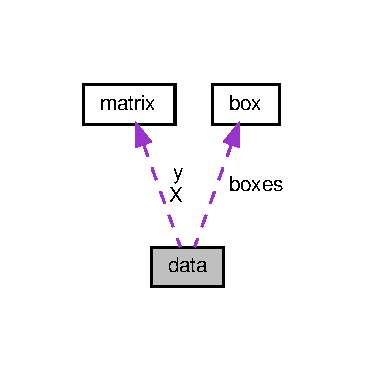
\includegraphics[width=177pt]{structdata__coll__graph}
\end{center}
\end{figure}
\subsection*{Public Attributes}
\begin{DoxyCompactItemize}
\item 
\mbox{\Hypertarget{structdata_a9de96028e1598b323d91ffb059cd48b2}\label{structdata_a9de96028e1598b323d91ffb059cd48b2}} 
int {\bfseries w}
\item 
\mbox{\Hypertarget{structdata_adbac4a041922ac9e6c47953f5fa23126}\label{structdata_adbac4a041922ac9e6c47953f5fa23126}} 
int {\bfseries h}
\item 
\mbox{\Hypertarget{structdata_a1f37ae26b26b12ef5c70a12957826e87}\label{structdata_a1f37ae26b26b12ef5c70a12957826e87}} 
\hyperlink{structmatrix}{matrix} {\bfseries X}
\item 
\mbox{\Hypertarget{structdata_a30946bde3a05e40df6fbb49c5dd9b627}\label{structdata_a30946bde3a05e40df6fbb49c5dd9b627}} 
\hyperlink{structmatrix}{matrix} {\bfseries y}
\item 
\mbox{\Hypertarget{structdata_a3ef4c4e942b1f2b6a5e64e7fb7e12491}\label{structdata_a3ef4c4e942b1f2b6a5e64e7fb7e12491}} 
int {\bfseries shallow}
\item 
\mbox{\Hypertarget{structdata_afba4d3b06050db7a30b0b11809ae6e23}\label{structdata_afba4d3b06050db7a30b0b11809ae6e23}} 
int $\ast$ {\bfseries num\+\_\+boxes}
\item 
\mbox{\Hypertarget{structdata_a8379df4ef55945c6fdb778dd581dce55}\label{structdata_a8379df4ef55945c6fdb778dd581dce55}} 
\hyperlink{structbox}{box} $\ast$$\ast$ {\bfseries boxes}
\end{DoxyCompactItemize}


The documentation for this struct was generated from the following file\+:\begin{DoxyCompactItemize}
\item 
darknet\+\_\+ros/darknet/include/darknet.\+h\end{DoxyCompactItemize}

\hypertarget{structdbox}{}\section{dbox Struct Reference}
\label{structdbox}\index{dbox@{dbox}}
\subsection*{Public Attributes}
\begin{DoxyCompactItemize}
\item 
\mbox{\Hypertarget{structdbox_af24e1ef9eae9dbcfefbcd86cc7ab342f}\label{structdbox_af24e1ef9eae9dbcfefbcd86cc7ab342f}} 
float {\bfseries dx}
\item 
\mbox{\Hypertarget{structdbox_acfa3fcbd522bc347d91b27229a935e1b}\label{structdbox_acfa3fcbd522bc347d91b27229a935e1b}} 
float {\bfseries dy}
\item 
\mbox{\Hypertarget{structdbox_a2d3a509dafd2b6c42326e0a008b1d929}\label{structdbox_a2d3a509dafd2b6c42326e0a008b1d929}} 
float {\bfseries dw}
\item 
\mbox{\Hypertarget{structdbox_a8321cbf92c464ba9c4eca5b8f0e9f48b}\label{structdbox_a8321cbf92c464ba9c4eca5b8f0e9f48b}} 
float {\bfseries dh}
\end{DoxyCompactItemize}


The documentation for this struct was generated from the following file\+:\begin{DoxyCompactItemize}
\item 
darknet\+\_\+ros/darknet/src/box.\+h\end{DoxyCompactItemize}

\hypertarget{structdetection}{}\section{detection Struct Reference}
\label{structdetection}\index{detection@{detection}}


Collaboration diagram for detection\+:
\nopagebreak
\begin{figure}[H]
\begin{center}
\leavevmode
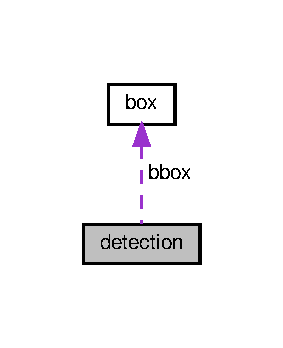
\includegraphics[width=136pt]{structdetection__coll__graph}
\end{center}
\end{figure}
\subsection*{Public Attributes}
\begin{DoxyCompactItemize}
\item 
\mbox{\Hypertarget{structdetection_a0e96ec314ffa1b5462b81752d1842191}\label{structdetection_a0e96ec314ffa1b5462b81752d1842191}} 
\hyperlink{structbox}{box} {\bfseries bbox}
\item 
\mbox{\Hypertarget{structdetection_a5501f226bdc7ce3630666a8065fa70b9}\label{structdetection_a5501f226bdc7ce3630666a8065fa70b9}} 
int {\bfseries classes}
\item 
\mbox{\Hypertarget{structdetection_a135fa8f73988691651cb54335e6e20c2}\label{structdetection_a135fa8f73988691651cb54335e6e20c2}} 
float $\ast$ {\bfseries prob}
\item 
\mbox{\Hypertarget{structdetection_a52d75f4c96f7ae42075f4792b1852946}\label{structdetection_a52d75f4c96f7ae42075f4792b1852946}} 
float $\ast$ {\bfseries mask}
\item 
\mbox{\Hypertarget{structdetection_afd81464803f6cca28d0d3171158f0d52}\label{structdetection_afd81464803f6cca28d0d3171158f0d52}} 
float {\bfseries objectness}
\item 
\mbox{\Hypertarget{structdetection_a134b1d6d4fa5b3356af1e4af9d53f344}\label{structdetection_a134b1d6d4fa5b3356af1e4af9d53f344}} 
int {\bfseries sort\+\_\+class}
\end{DoxyCompactItemize}


The documentation for this struct was generated from the following file\+:\begin{DoxyCompactItemize}
\item 
darknet\+\_\+ros/darknet/include/darknet.\+h\end{DoxyCompactItemize}

\hypertarget{structimage}{}\section{image Struct Reference}
\label{structimage}\index{image@{image}}
\subsection*{Public Attributes}
\begin{DoxyCompactItemize}
\item 
\mbox{\Hypertarget{structimage_aa6480e4024a0d5ca8d36b4145b3ceb43}\label{structimage_aa6480e4024a0d5ca8d36b4145b3ceb43}} 
int {\bfseries w}
\item 
\mbox{\Hypertarget{structimage_a30e2caee481a59608823b3bcec8a139f}\label{structimage_a30e2caee481a59608823b3bcec8a139f}} 
int {\bfseries h}
\item 
\mbox{\Hypertarget{structimage_aa67d2491c4d17dd240453d69dfc99482}\label{structimage_aa67d2491c4d17dd240453d69dfc99482}} 
int {\bfseries c}
\item 
\mbox{\Hypertarget{structimage_aed7e0704080213b735419d6661251a0a}\label{structimage_aed7e0704080213b735419d6661251a0a}} 
float $\ast$ {\bfseries data}
\end{DoxyCompactItemize}


The documentation for this struct was generated from the following file\+:\begin{DoxyCompactItemize}
\item 
darknet\+\_\+ros/darknet/include/darknet.\+h\end{DoxyCompactItemize}

\hypertarget{structkvp}{}\section{kvp Struct Reference}
\label{structkvp}\index{kvp@{kvp}}
\subsection*{Public Attributes}
\begin{DoxyCompactItemize}
\item 
\mbox{\Hypertarget{structkvp_ada553aa3459987ea43b7219868ba0a8f}\label{structkvp_ada553aa3459987ea43b7219868ba0a8f}} 
char $\ast$ {\bfseries key}
\item 
\mbox{\Hypertarget{structkvp_acfabb2665bc533f70cce1d708b6e6053}\label{structkvp_acfabb2665bc533f70cce1d708b6e6053}} 
char $\ast$ {\bfseries val}
\item 
\mbox{\Hypertarget{structkvp_a655effdf8a3be7aca94fe4f199f026fb}\label{structkvp_a655effdf8a3be7aca94fe4f199f026fb}} 
int {\bfseries used}
\end{DoxyCompactItemize}


The documentation for this struct was generated from the following file\+:\begin{DoxyCompactItemize}
\item 
darknet\+\_\+ros/darknet/src/option\+\_\+list.\+h\end{DoxyCompactItemize}

\hypertarget{structlayer}{}\section{layer Struct Reference}
\label{structlayer}\index{layer@{layer}}


Collaboration diagram for layer\+:\nopagebreak
\begin{figure}[H]
\begin{center}
\leavevmode
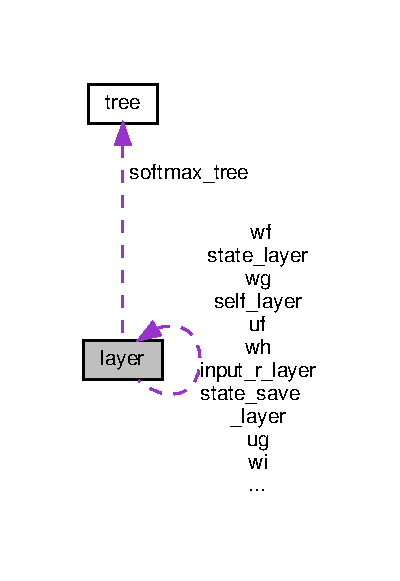
\includegraphics[width=192pt]{structlayer__coll__graph}
\end{center}
\end{figure}
\subsection*{Public Attributes}
\begin{DoxyCompactItemize}
\item 
\mbox{\Hypertarget{structlayer_af00e36adaf6e404a3e5234843c723714}\label{structlayer_af00e36adaf6e404a3e5234843c723714}} 
L\+A\+Y\+E\+R\+\_\+\+T\+Y\+PE {\bfseries type}
\item 
\mbox{\Hypertarget{structlayer_af7e837568a9975545159025b2fdbf31a}\label{structlayer_af7e837568a9975545159025b2fdbf31a}} 
A\+C\+T\+I\+V\+A\+T\+I\+ON {\bfseries activation}
\item 
\mbox{\Hypertarget{structlayer_a8f172c29b1ada15656f1f346e7491507}\label{structlayer_a8f172c29b1ada15656f1f346e7491507}} 
C\+O\+S\+T\+\_\+\+T\+Y\+PE {\bfseries cost\+\_\+type}
\item 
\mbox{\Hypertarget{structlayer_ad587958fc9c301a5987df7b3d68a09c1}\label{structlayer_ad587958fc9c301a5987df7b3d68a09c1}} 
void($\ast$ {\bfseries forward} )(struct \hyperlink{structlayer}{layer}, struct \hyperlink{structnetwork}{network})
\item 
\mbox{\Hypertarget{structlayer_a97391cfa71ea05cd917a3919f00e14a6}\label{structlayer_a97391cfa71ea05cd917a3919f00e14a6}} 
void($\ast$ {\bfseries backward} )(struct \hyperlink{structlayer}{layer}, struct \hyperlink{structnetwork}{network})
\item 
\mbox{\Hypertarget{structlayer_aefdbd48c48e52160fd806da7973de6e8}\label{structlayer_aefdbd48c48e52160fd806da7973de6e8}} 
void($\ast$ {\bfseries update} )(struct \hyperlink{structlayer}{layer}, \hyperlink{structupdate__args}{update\+\_\+args})
\item 
\mbox{\Hypertarget{structlayer_ae96ac4b6c9470848c52dddc95cb14b6a}\label{structlayer_ae96ac4b6c9470848c52dddc95cb14b6a}} 
void($\ast$ {\bfseries forward\+\_\+gpu} )(struct \hyperlink{structlayer}{layer}, struct \hyperlink{structnetwork}{network})
\item 
\mbox{\Hypertarget{structlayer_aedf9ba6db46b7291b41f424ff6346784}\label{structlayer_aedf9ba6db46b7291b41f424ff6346784}} 
void($\ast$ {\bfseries backward\+\_\+gpu} )(struct \hyperlink{structlayer}{layer}, struct \hyperlink{structnetwork}{network})
\item 
\mbox{\Hypertarget{structlayer_a820d8c7a9764dae29abe87e12f89b19e}\label{structlayer_a820d8c7a9764dae29abe87e12f89b19e}} 
void($\ast$ {\bfseries update\+\_\+gpu} )(struct \hyperlink{structlayer}{layer}, \hyperlink{structupdate__args}{update\+\_\+args})
\item 
\mbox{\Hypertarget{structlayer_a9af00a1fb4729a6ecdc62df42f4d3ae3}\label{structlayer_a9af00a1fb4729a6ecdc62df42f4d3ae3}} 
int {\bfseries batch\+\_\+normalize}
\item 
\mbox{\Hypertarget{structlayer_a84b1f1077ca914dafadb8e82bb12d46d}\label{structlayer_a84b1f1077ca914dafadb8e82bb12d46d}} 
int {\bfseries shortcut}
\item 
\mbox{\Hypertarget{structlayer_aff6bd99e74d13cccca4c492dd3e8de9c}\label{structlayer_aff6bd99e74d13cccca4c492dd3e8de9c}} 
int {\bfseries batch}
\item 
\mbox{\Hypertarget{structlayer_acf386a1f7b93955cc5d04513bb4e4649}\label{structlayer_acf386a1f7b93955cc5d04513bb4e4649}} 
int {\bfseries forced}
\item 
\mbox{\Hypertarget{structlayer_a44bd658c46a69f7863d781eb731475b0}\label{structlayer_a44bd658c46a69f7863d781eb731475b0}} 
int {\bfseries flipped}
\item 
\mbox{\Hypertarget{structlayer_a3fac583bf31e18ca679d195b1485b316}\label{structlayer_a3fac583bf31e18ca679d195b1485b316}} 
int {\bfseries inputs}
\item 
\mbox{\Hypertarget{structlayer_a0874fab782ae0e8f1075cc99d776478b}\label{structlayer_a0874fab782ae0e8f1075cc99d776478b}} 
int {\bfseries outputs}
\item 
\mbox{\Hypertarget{structlayer_a76a23567dbc4b223d8ba3c34c0f5e82f}\label{structlayer_a76a23567dbc4b223d8ba3c34c0f5e82f}} 
int {\bfseries nweights}
\item 
\mbox{\Hypertarget{structlayer_a8da8330f6a80f7fcb86fb2421c0484e5}\label{structlayer_a8da8330f6a80f7fcb86fb2421c0484e5}} 
int {\bfseries nbiases}
\item 
\mbox{\Hypertarget{structlayer_aaaa32102948bc9d4d4a506cf258b9910}\label{structlayer_aaaa32102948bc9d4d4a506cf258b9910}} 
int {\bfseries extra}
\item 
\mbox{\Hypertarget{structlayer_a086d4ebdf69d011ef4c11a487bd5ff60}\label{structlayer_a086d4ebdf69d011ef4c11a487bd5ff60}} 
int {\bfseries truths}
\item 
\mbox{\Hypertarget{structlayer_a7766d090f7dac8294b7456c1251ab485}\label{structlayer_a7766d090f7dac8294b7456c1251ab485}} 
int {\bfseries h}
\item 
\mbox{\Hypertarget{structlayer_a2e00450d79170c48791a1ed5a6f1d0c4}\label{structlayer_a2e00450d79170c48791a1ed5a6f1d0c4}} 
int {\bfseries w}
\item 
\mbox{\Hypertarget{structlayer_a6d10d2818541049ff11e94b257077a2d}\label{structlayer_a6d10d2818541049ff11e94b257077a2d}} 
int {\bfseries c}
\item 
\mbox{\Hypertarget{structlayer_a8f8224d0915a9903d93874aefe278f98}\label{structlayer_a8f8224d0915a9903d93874aefe278f98}} 
int {\bfseries out\+\_\+h}
\item 
\mbox{\Hypertarget{structlayer_a46454d978f2d84f8b8aba918a747c761}\label{structlayer_a46454d978f2d84f8b8aba918a747c761}} 
int {\bfseries out\+\_\+w}
\item 
\mbox{\Hypertarget{structlayer_a298d150dabc449824204579f4851b926}\label{structlayer_a298d150dabc449824204579f4851b926}} 
int {\bfseries out\+\_\+c}
\item 
\mbox{\Hypertarget{structlayer_a454b8980d0186eb0095a25aadef41744}\label{structlayer_a454b8980d0186eb0095a25aadef41744}} 
int {\bfseries n}
\item 
\mbox{\Hypertarget{structlayer_a97f045f2c42981c7d1b9e47b8c69788f}\label{structlayer_a97f045f2c42981c7d1b9e47b8c69788f}} 
int {\bfseries max\+\_\+boxes}
\item 
\mbox{\Hypertarget{structlayer_a2a7404991ccfcc0b7b884a7638d078ff}\label{structlayer_a2a7404991ccfcc0b7b884a7638d078ff}} 
int {\bfseries groups}
\item 
\mbox{\Hypertarget{structlayer_a4168fc846264723c6149d4e464097a00}\label{structlayer_a4168fc846264723c6149d4e464097a00}} 
int {\bfseries size}
\item 
\mbox{\Hypertarget{structlayer_a0286d4acb9afd3c080b0158bf6ef3ca1}\label{structlayer_a0286d4acb9afd3c080b0158bf6ef3ca1}} 
int {\bfseries side}
\item 
\mbox{\Hypertarget{structlayer_a239bfd11f56b41f70e2933333f80c81b}\label{structlayer_a239bfd11f56b41f70e2933333f80c81b}} 
int {\bfseries stride}
\item 
\mbox{\Hypertarget{structlayer_abf6e12515b8a316fb280c43234701022}\label{structlayer_abf6e12515b8a316fb280c43234701022}} 
int {\bfseries reverse}
\item 
\mbox{\Hypertarget{structlayer_abd9dc10c7124e7d7e54b3ad6811deb00}\label{structlayer_abd9dc10c7124e7d7e54b3ad6811deb00}} 
int {\bfseries flatten}
\item 
\mbox{\Hypertarget{structlayer_aeca00102f8c93bcb3e30670623e835de}\label{structlayer_aeca00102f8c93bcb3e30670623e835de}} 
int {\bfseries spatial}
\item 
\mbox{\Hypertarget{structlayer_ac7f6c035a8161713696db818f4dcb6ea}\label{structlayer_ac7f6c035a8161713696db818f4dcb6ea}} 
int {\bfseries pad}
\item 
\mbox{\Hypertarget{structlayer_a30e95ebb753b16822e759bd903ca8f1a}\label{structlayer_a30e95ebb753b16822e759bd903ca8f1a}} 
int {\bfseries sqrt}
\item 
\mbox{\Hypertarget{structlayer_ade1cdfc041b6c641c73f74bea2492b5f}\label{structlayer_ade1cdfc041b6c641c73f74bea2492b5f}} 
int {\bfseries flip}
\item 
\mbox{\Hypertarget{structlayer_a98964b626e3a83be1235c3aed8178810}\label{structlayer_a98964b626e3a83be1235c3aed8178810}} 
int {\bfseries index}
\item 
\mbox{\Hypertarget{structlayer_a7a6777b89f1faa3ec8dbc9d6fd2b431b}\label{structlayer_a7a6777b89f1faa3ec8dbc9d6fd2b431b}} 
int {\bfseries binary}
\item 
\mbox{\Hypertarget{structlayer_abd05a6404f54ecf89e6ddc0c23d431ab}\label{structlayer_abd05a6404f54ecf89e6ddc0c23d431ab}} 
int {\bfseries xnor}
\item 
\mbox{\Hypertarget{structlayer_ad060e2cc161c5aa290a76613d024f03a}\label{structlayer_ad060e2cc161c5aa290a76613d024f03a}} 
int {\bfseries steps}
\item 
\mbox{\Hypertarget{structlayer_a10071bf2848df19c845b55fc575dcd9c}\label{structlayer_a10071bf2848df19c845b55fc575dcd9c}} 
int {\bfseries hidden}
\item 
\mbox{\Hypertarget{structlayer_ac669e3f8294d93e118977cec91bb792b}\label{structlayer_ac669e3f8294d93e118977cec91bb792b}} 
int {\bfseries truth}
\item 
\mbox{\Hypertarget{structlayer_a4ecd91c02a2368b51bdfa66d3b92c6d6}\label{structlayer_a4ecd91c02a2368b51bdfa66d3b92c6d6}} 
float {\bfseries smooth}
\item 
\mbox{\Hypertarget{structlayer_aaf67b912e38bb35777c7dd1867217a06}\label{structlayer_aaf67b912e38bb35777c7dd1867217a06}} 
float {\bfseries dot}
\item 
\mbox{\Hypertarget{structlayer_ad484c9f3947a86cd9c328811c1d0b24f}\label{structlayer_ad484c9f3947a86cd9c328811c1d0b24f}} 
float {\bfseries angle}
\item 
\mbox{\Hypertarget{structlayer_a5a580dce2dc1716ff9fe8524da2f4237}\label{structlayer_a5a580dce2dc1716ff9fe8524da2f4237}} 
float {\bfseries jitter}
\item 
\mbox{\Hypertarget{structlayer_a900c449abe20f24a3ab6f171679d12dd}\label{structlayer_a900c449abe20f24a3ab6f171679d12dd}} 
float {\bfseries saturation}
\item 
\mbox{\Hypertarget{structlayer_a3c8781cb592ce45d1a6e331e558310f7}\label{structlayer_a3c8781cb592ce45d1a6e331e558310f7}} 
float {\bfseries exposure}
\item 
\mbox{\Hypertarget{structlayer_a67d23cb25a1d405a4cc63bdea8363f78}\label{structlayer_a67d23cb25a1d405a4cc63bdea8363f78}} 
float {\bfseries shift}
\item 
\mbox{\Hypertarget{structlayer_a2752501fc00b1ff2bdd19e0a24b5370c}\label{structlayer_a2752501fc00b1ff2bdd19e0a24b5370c}} 
float {\bfseries ratio}
\item 
\mbox{\Hypertarget{structlayer_a329f298275a866fae317080159336d98}\label{structlayer_a329f298275a866fae317080159336d98}} 
float {\bfseries learning\+\_\+rate\+\_\+scale}
\item 
\mbox{\Hypertarget{structlayer_a1728042fca5440265c959059a869bd2f}\label{structlayer_a1728042fca5440265c959059a869bd2f}} 
float {\bfseries clip}
\item 
\mbox{\Hypertarget{structlayer_a7b07ddac3afad25586ff7c18956ba9a9}\label{structlayer_a7b07ddac3afad25586ff7c18956ba9a9}} 
int {\bfseries softmax}
\item 
\mbox{\Hypertarget{structlayer_af8d01e54a44d8682c38d431c32faed45}\label{structlayer_af8d01e54a44d8682c38d431c32faed45}} 
int {\bfseries classes}
\item 
\mbox{\Hypertarget{structlayer_a6b8636464bcea5dea2c2235ee133af29}\label{structlayer_a6b8636464bcea5dea2c2235ee133af29}} 
int {\bfseries coords}
\item 
\mbox{\Hypertarget{structlayer_a509601d552c5e188902dc7cfddfe6ee4}\label{structlayer_a509601d552c5e188902dc7cfddfe6ee4}} 
int {\bfseries background}
\item 
\mbox{\Hypertarget{structlayer_a662867ba4218e923a302fd215dab2ddd}\label{structlayer_a662867ba4218e923a302fd215dab2ddd}} 
int {\bfseries rescore}
\item 
\mbox{\Hypertarget{structlayer_aaf0a24ead54282e6bbb9c766f357c57f}\label{structlayer_aaf0a24ead54282e6bbb9c766f357c57f}} 
int {\bfseries objectness}
\item 
\mbox{\Hypertarget{structlayer_aac680bb3fa86a374a0252fff77bb887d}\label{structlayer_aac680bb3fa86a374a0252fff77bb887d}} 
int {\bfseries joint}
\item 
\mbox{\Hypertarget{structlayer_addd7dd5ca8a7ce6bb15aa2d06efe69ee}\label{structlayer_addd7dd5ca8a7ce6bb15aa2d06efe69ee}} 
int {\bfseries noadjust}
\item 
\mbox{\Hypertarget{structlayer_a13f7dcacfefce8f8f5694dad9e5aa6ae}\label{structlayer_a13f7dcacfefce8f8f5694dad9e5aa6ae}} 
int {\bfseries reorg}
\item 
\mbox{\Hypertarget{structlayer_a540b5bcf6b30bef535ff82e133bffd79}\label{structlayer_a540b5bcf6b30bef535ff82e133bffd79}} 
int {\bfseries log}
\item 
\mbox{\Hypertarget{structlayer_a386df76b9ede3725ade44f66c45ecdcb}\label{structlayer_a386df76b9ede3725ade44f66c45ecdcb}} 
int {\bfseries tanh}
\item 
\mbox{\Hypertarget{structlayer_aaa82c8e027d08dfd571c663653f85588}\label{structlayer_aaa82c8e027d08dfd571c663653f85588}} 
int $\ast$ {\bfseries mask}
\item 
\mbox{\Hypertarget{structlayer_a5899baa591f5d9e897b6af62b0fd13e0}\label{structlayer_a5899baa591f5d9e897b6af62b0fd13e0}} 
int {\bfseries total}
\item 
\mbox{\Hypertarget{structlayer_aa9495e20d42d431aa52dd4eedb03e8b5}\label{structlayer_aa9495e20d42d431aa52dd4eedb03e8b5}} 
float {\bfseries alpha}
\item 
\mbox{\Hypertarget{structlayer_a375acd63c42b47b9c3007a1c064caef7}\label{structlayer_a375acd63c42b47b9c3007a1c064caef7}} 
float {\bfseries beta}
\item 
\mbox{\Hypertarget{structlayer_ac8ee04d5346e8f3d682ebc02e8a6b663}\label{structlayer_ac8ee04d5346e8f3d682ebc02e8a6b663}} 
float {\bfseries kappa}
\item 
\mbox{\Hypertarget{structlayer_a4cb681c94203182c328d7818bcb39de8}\label{structlayer_a4cb681c94203182c328d7818bcb39de8}} 
float {\bfseries coord\+\_\+scale}
\item 
\mbox{\Hypertarget{structlayer_a502c7f71d253c01f1724adbe8bc585fc}\label{structlayer_a502c7f71d253c01f1724adbe8bc585fc}} 
float {\bfseries object\+\_\+scale}
\item 
\mbox{\Hypertarget{structlayer_ad10b4f2f32b1991c3cd8e66d138c5eaa}\label{structlayer_ad10b4f2f32b1991c3cd8e66d138c5eaa}} 
float {\bfseries noobject\+\_\+scale}
\item 
\mbox{\Hypertarget{structlayer_a9e6e9d0cbdfbef34920e842d0542670e}\label{structlayer_a9e6e9d0cbdfbef34920e842d0542670e}} 
float {\bfseries mask\+\_\+scale}
\item 
\mbox{\Hypertarget{structlayer_a7175af778d4be5a066ccc212421617b7}\label{structlayer_a7175af778d4be5a066ccc212421617b7}} 
float {\bfseries class\+\_\+scale}
\item 
\mbox{\Hypertarget{structlayer_a9f5919edff3bdaa0e3f02f13728415c3}\label{structlayer_a9f5919edff3bdaa0e3f02f13728415c3}} 
int {\bfseries bias\+\_\+match}
\item 
\mbox{\Hypertarget{structlayer_a411feca89284377c83dd97141540dd83}\label{structlayer_a411feca89284377c83dd97141540dd83}} 
int {\bfseries random}
\item 
\mbox{\Hypertarget{structlayer_ad1052957257631f1cba42a25ed63159b}\label{structlayer_ad1052957257631f1cba42a25ed63159b}} 
float {\bfseries ignore\+\_\+thresh}
\item 
\mbox{\Hypertarget{structlayer_a53f9de692e18bf39eeaf322afa9612cb}\label{structlayer_a53f9de692e18bf39eeaf322afa9612cb}} 
float {\bfseries truth\+\_\+thresh}
\item 
\mbox{\Hypertarget{structlayer_a20c059ef419e2b863c67d4df87ec4488}\label{structlayer_a20c059ef419e2b863c67d4df87ec4488}} 
float {\bfseries thresh}
\item 
\mbox{\Hypertarget{structlayer_afa6d90f3ca746a776b5d79b3f8ead52d}\label{structlayer_afa6d90f3ca746a776b5d79b3f8ead52d}} 
float {\bfseries focus}
\item 
\mbox{\Hypertarget{structlayer_a510630027ff3061ae0ad07e151fbf1a5}\label{structlayer_a510630027ff3061ae0ad07e151fbf1a5}} 
int {\bfseries classfix}
\item 
\mbox{\Hypertarget{structlayer_afe0cd75c5d7d210ec413df79b73aa40a}\label{structlayer_afe0cd75c5d7d210ec413df79b73aa40a}} 
int {\bfseries absolute}
\item 
\mbox{\Hypertarget{structlayer_a975a97f550b56c3503feba36b8eacf45}\label{structlayer_a975a97f550b56c3503feba36b8eacf45}} 
int {\bfseries onlyforward}
\item 
\mbox{\Hypertarget{structlayer_ada9c281fad0eae687276387e0dc5d8d1}\label{structlayer_ada9c281fad0eae687276387e0dc5d8d1}} 
int {\bfseries stopbackward}
\item 
\mbox{\Hypertarget{structlayer_a90d11f2ddc0ae1f0bfcce33d5eab9f1b}\label{structlayer_a90d11f2ddc0ae1f0bfcce33d5eab9f1b}} 
int {\bfseries dontload}
\item 
\mbox{\Hypertarget{structlayer_acc28d07d2164bd944a3a3857b482629d}\label{structlayer_acc28d07d2164bd944a3a3857b482629d}} 
int {\bfseries dontsave}
\item 
\mbox{\Hypertarget{structlayer_a5ba6e7bfc48b309721ddbed942d2d531}\label{structlayer_a5ba6e7bfc48b309721ddbed942d2d531}} 
int {\bfseries dontloadscales}
\item 
\mbox{\Hypertarget{structlayer_a965290dca263c7774c9e9b4272a43c49}\label{structlayer_a965290dca263c7774c9e9b4272a43c49}} 
float {\bfseries temperature}
\item 
\mbox{\Hypertarget{structlayer_a3c133867d28268532e3786ae75db47fc}\label{structlayer_a3c133867d28268532e3786ae75db47fc}} 
float {\bfseries probability}
\item 
\mbox{\Hypertarget{structlayer_a7225a2fa7d8cf13688e1c8a421f3ad7f}\label{structlayer_a7225a2fa7d8cf13688e1c8a421f3ad7f}} 
float {\bfseries scale}
\item 
\mbox{\Hypertarget{structlayer_a5a1da440e0ebe63674288f9006bd8ad7}\label{structlayer_a5a1da440e0ebe63674288f9006bd8ad7}} 
char $\ast$ {\bfseries cweights}
\item 
\mbox{\Hypertarget{structlayer_a545ce2f1db475b370db778c433913fde}\label{structlayer_a545ce2f1db475b370db778c433913fde}} 
int $\ast$ {\bfseries indexes}
\item 
\mbox{\Hypertarget{structlayer_afd5797d71336f51f9b5b1bd1ef0bddd8}\label{structlayer_afd5797d71336f51f9b5b1bd1ef0bddd8}} 
int $\ast$ {\bfseries input\+\_\+layers}
\item 
\mbox{\Hypertarget{structlayer_aef52d6a821c836ddd1b1993911c648f2}\label{structlayer_aef52d6a821c836ddd1b1993911c648f2}} 
int $\ast$ {\bfseries input\+\_\+sizes}
\item 
\mbox{\Hypertarget{structlayer_a9950b1b44120256269e082cb5efbd42e}\label{structlayer_a9950b1b44120256269e082cb5efbd42e}} 
int $\ast$ {\bfseries map}
\item 
\mbox{\Hypertarget{structlayer_a254a888ee1b4383a7ce6035a88e7b825}\label{structlayer_a254a888ee1b4383a7ce6035a88e7b825}} 
float $\ast$ {\bfseries rand}
\item 
\mbox{\Hypertarget{structlayer_a9a71dbf0ad70f63a10787d8217633776}\label{structlayer_a9a71dbf0ad70f63a10787d8217633776}} 
float $\ast$ {\bfseries cost}
\item 
\mbox{\Hypertarget{structlayer_af47d59ee97d2b512e5ca64a25af476c1}\label{structlayer_af47d59ee97d2b512e5ca64a25af476c1}} 
float $\ast$ {\bfseries state}
\item 
\mbox{\Hypertarget{structlayer_aa82477e38a85af20ebd0300cab6ea6e1}\label{structlayer_aa82477e38a85af20ebd0300cab6ea6e1}} 
float $\ast$ {\bfseries prev\+\_\+state}
\item 
\mbox{\Hypertarget{structlayer_a8c96fb4f8b4a7d7dac14d6220938bdc3}\label{structlayer_a8c96fb4f8b4a7d7dac14d6220938bdc3}} 
float $\ast$ {\bfseries forgot\+\_\+state}
\item 
\mbox{\Hypertarget{structlayer_a03015ecf4e0ca81f3b0133c93cab1354}\label{structlayer_a03015ecf4e0ca81f3b0133c93cab1354}} 
float $\ast$ {\bfseries forgot\+\_\+delta}
\item 
\mbox{\Hypertarget{structlayer_a48c287c5df2e2cd3bea497e6a93487a6}\label{structlayer_a48c287c5df2e2cd3bea497e6a93487a6}} 
float $\ast$ {\bfseries state\+\_\+delta}
\item 
\mbox{\Hypertarget{structlayer_abf10dce2bd742799a95eb1241e0c4e71}\label{structlayer_abf10dce2bd742799a95eb1241e0c4e71}} 
float $\ast$ {\bfseries combine\+\_\+cpu}
\item 
\mbox{\Hypertarget{structlayer_a00fca0bda761ca0a2ceaf81934b31293}\label{structlayer_a00fca0bda761ca0a2ceaf81934b31293}} 
float $\ast$ {\bfseries combine\+\_\+delta\+\_\+cpu}
\item 
\mbox{\Hypertarget{structlayer_aa2edc68cb4713d7b34f52b27b2c0a35b}\label{structlayer_aa2edc68cb4713d7b34f52b27b2c0a35b}} 
float $\ast$ {\bfseries concat}
\item 
\mbox{\Hypertarget{structlayer_a1de4fac7dfc2c7c9ab387bc322246258}\label{structlayer_a1de4fac7dfc2c7c9ab387bc322246258}} 
float $\ast$ {\bfseries concat\+\_\+delta}
\item 
\mbox{\Hypertarget{structlayer_a105fc98c2adbd8d8de839e327fb284b7}\label{structlayer_a105fc98c2adbd8d8de839e327fb284b7}} 
float $\ast$ {\bfseries binary\+\_\+weights}
\item 
\mbox{\Hypertarget{structlayer_aaa7f20cb294d09ee0011d32658675a48}\label{structlayer_aaa7f20cb294d09ee0011d32658675a48}} 
float $\ast$ {\bfseries biases}
\item 
\mbox{\Hypertarget{structlayer_a53f11ac2a72b28b8c3529b799f1662fd}\label{structlayer_a53f11ac2a72b28b8c3529b799f1662fd}} 
float $\ast$ {\bfseries bias\+\_\+updates}
\item 
\mbox{\Hypertarget{structlayer_a82237cebb237c586f13f0a0ab35e38a3}\label{structlayer_a82237cebb237c586f13f0a0ab35e38a3}} 
float $\ast$ {\bfseries scales}
\item 
\mbox{\Hypertarget{structlayer_afe8abd57f459714570b99b521cf9e159}\label{structlayer_afe8abd57f459714570b99b521cf9e159}} 
float $\ast$ {\bfseries scale\+\_\+updates}
\item 
\mbox{\Hypertarget{structlayer_a552e6eca39a5d0dc6fa12901502c7e78}\label{structlayer_a552e6eca39a5d0dc6fa12901502c7e78}} 
float $\ast$ {\bfseries weights}
\item 
\mbox{\Hypertarget{structlayer_a24eda1775cf0b0e188446089a25780b7}\label{structlayer_a24eda1775cf0b0e188446089a25780b7}} 
float $\ast$ {\bfseries weight\+\_\+updates}
\item 
\mbox{\Hypertarget{structlayer_a1360cf3c28df067cc6f3af139fa95d3a}\label{structlayer_a1360cf3c28df067cc6f3af139fa95d3a}} 
float $\ast$ {\bfseries delta}
\item 
\mbox{\Hypertarget{structlayer_a04d23c71428242b3153eda588f844eb3}\label{structlayer_a04d23c71428242b3153eda588f844eb3}} 
float $\ast$ {\bfseries output}
\item 
\mbox{\Hypertarget{structlayer_a6554389eac1170d557224124d81eb3d6}\label{structlayer_a6554389eac1170d557224124d81eb3d6}} 
float $\ast$ {\bfseries loss}
\item 
\mbox{\Hypertarget{structlayer_ae8ed52c73d5fc1d13d2fbf0b920dda7e}\label{structlayer_ae8ed52c73d5fc1d13d2fbf0b920dda7e}} 
float $\ast$ {\bfseries squared}
\item 
\mbox{\Hypertarget{structlayer_acb730788dd9a0c77c7e501b9118a2933}\label{structlayer_acb730788dd9a0c77c7e501b9118a2933}} 
float $\ast$ {\bfseries norms}
\item 
\mbox{\Hypertarget{structlayer_ac3167d1999c93f60856076a4da9c3fc3}\label{structlayer_ac3167d1999c93f60856076a4da9c3fc3}} 
float $\ast$ {\bfseries spatial\+\_\+mean}
\item 
\mbox{\Hypertarget{structlayer_a57e3ce10060c51c846086d20944f2448}\label{structlayer_a57e3ce10060c51c846086d20944f2448}} 
float $\ast$ {\bfseries mean}
\item 
\mbox{\Hypertarget{structlayer_a4307e89c5c91bef35a9b54e4662e247d}\label{structlayer_a4307e89c5c91bef35a9b54e4662e247d}} 
float $\ast$ {\bfseries variance}
\item 
\mbox{\Hypertarget{structlayer_a6ae807c0129ad454f9a850e2e5c20544}\label{structlayer_a6ae807c0129ad454f9a850e2e5c20544}} 
float $\ast$ {\bfseries mean\+\_\+delta}
\item 
\mbox{\Hypertarget{structlayer_a6ac77051b9f79c2a72732b7b7f3f536c}\label{structlayer_a6ac77051b9f79c2a72732b7b7f3f536c}} 
float $\ast$ {\bfseries variance\+\_\+delta}
\item 
\mbox{\Hypertarget{structlayer_aadc24d03a6dbab21fcafad3d29bb1310}\label{structlayer_aadc24d03a6dbab21fcafad3d29bb1310}} 
float $\ast$ {\bfseries rolling\+\_\+mean}
\item 
\mbox{\Hypertarget{structlayer_a316830907cb724b9304cea311c8d8dc5}\label{structlayer_a316830907cb724b9304cea311c8d8dc5}} 
float $\ast$ {\bfseries rolling\+\_\+variance}
\item 
\mbox{\Hypertarget{structlayer_a78b279684acc59b1b891f63225e5715e}\label{structlayer_a78b279684acc59b1b891f63225e5715e}} 
float $\ast$ {\bfseries x}
\item 
\mbox{\Hypertarget{structlayer_a080a015b7c11489ecca087ece911a6b6}\label{structlayer_a080a015b7c11489ecca087ece911a6b6}} 
float $\ast$ {\bfseries x\+\_\+norm}
\item 
\mbox{\Hypertarget{structlayer_acfd875ae4a4c774d30e04e03a24085f9}\label{structlayer_acfd875ae4a4c774d30e04e03a24085f9}} 
float $\ast$ {\bfseries m}
\item 
\mbox{\Hypertarget{structlayer_a9493ddf18d4f6d9234a703d2575697db}\label{structlayer_a9493ddf18d4f6d9234a703d2575697db}} 
float $\ast$ {\bfseries v}
\item 
\mbox{\Hypertarget{structlayer_acfe31e9816074f6118b1dfaa7c55e53f}\label{structlayer_acfe31e9816074f6118b1dfaa7c55e53f}} 
float $\ast$ {\bfseries bias\+\_\+m}
\item 
\mbox{\Hypertarget{structlayer_a52052221eb80a84d1486c79ede9a1477}\label{structlayer_a52052221eb80a84d1486c79ede9a1477}} 
float $\ast$ {\bfseries bias\+\_\+v}
\item 
\mbox{\Hypertarget{structlayer_a858dcb301c88b816430a797dce3b95b6}\label{structlayer_a858dcb301c88b816430a797dce3b95b6}} 
float $\ast$ {\bfseries scale\+\_\+m}
\item 
\mbox{\Hypertarget{structlayer_a881162ac744dcf116ec9c14c97fb1633}\label{structlayer_a881162ac744dcf116ec9c14c97fb1633}} 
float $\ast$ {\bfseries scale\+\_\+v}
\item 
\mbox{\Hypertarget{structlayer_aa38a67974b34aad9ada08b970ace3318}\label{structlayer_aa38a67974b34aad9ada08b970ace3318}} 
float $\ast$ {\bfseries z\+\_\+cpu}
\item 
\mbox{\Hypertarget{structlayer_aaaefd9c6dccae5505e5600831d99a026}\label{structlayer_aaaefd9c6dccae5505e5600831d99a026}} 
float $\ast$ {\bfseries r\+\_\+cpu}
\item 
\mbox{\Hypertarget{structlayer_aff93d520e69e75d6aa104a687d5ab21e}\label{structlayer_aff93d520e69e75d6aa104a687d5ab21e}} 
float $\ast$ {\bfseries h\+\_\+cpu}
\item 
\mbox{\Hypertarget{structlayer_afcadbe531d4b320c23877019284168b0}\label{structlayer_afcadbe531d4b320c23877019284168b0}} 
float $\ast$ {\bfseries prev\+\_\+state\+\_\+cpu}
\item 
\mbox{\Hypertarget{structlayer_a8a566c099cbba1da8bb7cc4d90643d0b}\label{structlayer_a8a566c099cbba1da8bb7cc4d90643d0b}} 
float $\ast$ {\bfseries temp\+\_\+cpu}
\item 
\mbox{\Hypertarget{structlayer_a12c40b990c72966e93dc2936c5a91447}\label{structlayer_a12c40b990c72966e93dc2936c5a91447}} 
float $\ast$ {\bfseries temp2\+\_\+cpu}
\item 
\mbox{\Hypertarget{structlayer_a5576a957c950547134d305cb5e7ed42b}\label{structlayer_a5576a957c950547134d305cb5e7ed42b}} 
float $\ast$ {\bfseries temp3\+\_\+cpu}
\item 
\mbox{\Hypertarget{structlayer_acb9dec30688fb0f1d836e14e507a441d}\label{structlayer_acb9dec30688fb0f1d836e14e507a441d}} 
float $\ast$ {\bfseries dh\+\_\+cpu}
\item 
\mbox{\Hypertarget{structlayer_af62005e5700299a59c76dafe7bb00529}\label{structlayer_af62005e5700299a59c76dafe7bb00529}} 
float $\ast$ {\bfseries hh\+\_\+cpu}
\item 
\mbox{\Hypertarget{structlayer_a4844271cfffe336d89a934705c8e3cc9}\label{structlayer_a4844271cfffe336d89a934705c8e3cc9}} 
float $\ast$ {\bfseries prev\+\_\+cell\+\_\+cpu}
\item 
\mbox{\Hypertarget{structlayer_a0dbcc8d653aaea58b9aaddcda570b9fb}\label{structlayer_a0dbcc8d653aaea58b9aaddcda570b9fb}} 
float $\ast$ {\bfseries cell\+\_\+cpu}
\item 
\mbox{\Hypertarget{structlayer_a2f326ac879fefe2ab4ef8a4b48664b01}\label{structlayer_a2f326ac879fefe2ab4ef8a4b48664b01}} 
float $\ast$ {\bfseries f\+\_\+cpu}
\item 
\mbox{\Hypertarget{structlayer_a3cbe33860e4b1605034034f9dbddc227}\label{structlayer_a3cbe33860e4b1605034034f9dbddc227}} 
float $\ast$ {\bfseries i\+\_\+cpu}
\item 
\mbox{\Hypertarget{structlayer_abc8c1af0663167cc50b83e918e0a3c1d}\label{structlayer_abc8c1af0663167cc50b83e918e0a3c1d}} 
float $\ast$ {\bfseries g\+\_\+cpu}
\item 
\mbox{\Hypertarget{structlayer_ae0b82851bad0a9588a448e93bf6ba5cc}\label{structlayer_ae0b82851bad0a9588a448e93bf6ba5cc}} 
float $\ast$ {\bfseries o\+\_\+cpu}
\item 
\mbox{\Hypertarget{structlayer_ae6b07fa9262cecce9ec149e37c001d81}\label{structlayer_ae6b07fa9262cecce9ec149e37c001d81}} 
float $\ast$ {\bfseries c\+\_\+cpu}
\item 
\mbox{\Hypertarget{structlayer_ac4bc1b441b4be3b7a33d48934d883a92}\label{structlayer_ac4bc1b441b4be3b7a33d48934d883a92}} 
float $\ast$ {\bfseries dc\+\_\+cpu}
\item 
\mbox{\Hypertarget{structlayer_a65b3a401a9e02fc7b7260705ade1b317}\label{structlayer_a65b3a401a9e02fc7b7260705ade1b317}} 
float $\ast$ {\bfseries binary\+\_\+input}
\item 
\mbox{\Hypertarget{structlayer_afcfa8ab43a850ea490c6d82ff05def87}\label{structlayer_afcfa8ab43a850ea490c6d82ff05def87}} 
struct \hyperlink{structlayer}{layer} $\ast$ {\bfseries input\+\_\+layer}
\item 
\mbox{\Hypertarget{structlayer_a4b265f84aaca806ccaf8607156fbb067}\label{structlayer_a4b265f84aaca806ccaf8607156fbb067}} 
struct \hyperlink{structlayer}{layer} $\ast$ {\bfseries self\+\_\+layer}
\item 
\mbox{\Hypertarget{structlayer_a93e590cb5d7d1cb0ff4803cd15dd0b51}\label{structlayer_a93e590cb5d7d1cb0ff4803cd15dd0b51}} 
struct \hyperlink{structlayer}{layer} $\ast$ {\bfseries output\+\_\+layer}
\item 
\mbox{\Hypertarget{structlayer_a091a5757286a08a99ee76cd332ae8631}\label{structlayer_a091a5757286a08a99ee76cd332ae8631}} 
struct \hyperlink{structlayer}{layer} $\ast$ {\bfseries reset\+\_\+layer}
\item 
\mbox{\Hypertarget{structlayer_a777da8634fb7e1e1243c79dbec93304e}\label{structlayer_a777da8634fb7e1e1243c79dbec93304e}} 
struct \hyperlink{structlayer}{layer} $\ast$ {\bfseries update\+\_\+layer}
\item 
\mbox{\Hypertarget{structlayer_ac79543fef7f4662508f07bc68483a78f}\label{structlayer_ac79543fef7f4662508f07bc68483a78f}} 
struct \hyperlink{structlayer}{layer} $\ast$ {\bfseries state\+\_\+layer}
\item 
\mbox{\Hypertarget{structlayer_ad7cd67a8989bbdafa89982d9c1f64c78}\label{structlayer_ad7cd67a8989bbdafa89982d9c1f64c78}} 
struct \hyperlink{structlayer}{layer} $\ast$ {\bfseries input\+\_\+gate\+\_\+layer}
\item 
\mbox{\Hypertarget{structlayer_a0b1b6cbee3d9421055512d52d8291929}\label{structlayer_a0b1b6cbee3d9421055512d52d8291929}} 
struct \hyperlink{structlayer}{layer} $\ast$ {\bfseries state\+\_\+gate\+\_\+layer}
\item 
\mbox{\Hypertarget{structlayer_a1dca5c6d106ae9a60fe70b7a9532cfc5}\label{structlayer_a1dca5c6d106ae9a60fe70b7a9532cfc5}} 
struct \hyperlink{structlayer}{layer} $\ast$ {\bfseries input\+\_\+save\+\_\+layer}
\item 
\mbox{\Hypertarget{structlayer_a5258c642da20d6011c579edc4d1efe03}\label{structlayer_a5258c642da20d6011c579edc4d1efe03}} 
struct \hyperlink{structlayer}{layer} $\ast$ {\bfseries state\+\_\+save\+\_\+layer}
\item 
\mbox{\Hypertarget{structlayer_a1f41820898325961a6acc16b113b90c7}\label{structlayer_a1f41820898325961a6acc16b113b90c7}} 
struct \hyperlink{structlayer}{layer} $\ast$ {\bfseries input\+\_\+state\+\_\+layer}
\item 
\mbox{\Hypertarget{structlayer_a2c2e848a9857ec5f5fd2b6205b2e963f}\label{structlayer_a2c2e848a9857ec5f5fd2b6205b2e963f}} 
struct \hyperlink{structlayer}{layer} $\ast$ {\bfseries state\+\_\+state\+\_\+layer}
\item 
\mbox{\Hypertarget{structlayer_addf22ace8c49b848e3f19122bdb703d5}\label{structlayer_addf22ace8c49b848e3f19122bdb703d5}} 
struct \hyperlink{structlayer}{layer} $\ast$ {\bfseries input\+\_\+z\+\_\+layer}
\item 
\mbox{\Hypertarget{structlayer_a22598554a0e6c65dd6e6fb2246ceb6cf}\label{structlayer_a22598554a0e6c65dd6e6fb2246ceb6cf}} 
struct \hyperlink{structlayer}{layer} $\ast$ {\bfseries state\+\_\+z\+\_\+layer}
\item 
\mbox{\Hypertarget{structlayer_a7c67ff6cd710e56e2eb0da199c4d0cff}\label{structlayer_a7c67ff6cd710e56e2eb0da199c4d0cff}} 
struct \hyperlink{structlayer}{layer} $\ast$ {\bfseries input\+\_\+r\+\_\+layer}
\item 
\mbox{\Hypertarget{structlayer_a2ce6e1f069b4ebc57b4a49d56afbe875}\label{structlayer_a2ce6e1f069b4ebc57b4a49d56afbe875}} 
struct \hyperlink{structlayer}{layer} $\ast$ {\bfseries state\+\_\+r\+\_\+layer}
\item 
\mbox{\Hypertarget{structlayer_a526089c1cc0aa9d9738f3e5b8358166f}\label{structlayer_a526089c1cc0aa9d9738f3e5b8358166f}} 
struct \hyperlink{structlayer}{layer} $\ast$ {\bfseries input\+\_\+h\+\_\+layer}
\item 
\mbox{\Hypertarget{structlayer_a8d566da721348636889c3f9aadd6f5e0}\label{structlayer_a8d566da721348636889c3f9aadd6f5e0}} 
struct \hyperlink{structlayer}{layer} $\ast$ {\bfseries state\+\_\+h\+\_\+layer}
\item 
\mbox{\Hypertarget{structlayer_af5ebb2f94c441e094e4ba3f04e318185}\label{structlayer_af5ebb2f94c441e094e4ba3f04e318185}} 
struct \hyperlink{structlayer}{layer} $\ast$ {\bfseries wz}
\item 
\mbox{\Hypertarget{structlayer_aebc50a1f698ed78ce6ca500609ad7308}\label{structlayer_aebc50a1f698ed78ce6ca500609ad7308}} 
struct \hyperlink{structlayer}{layer} $\ast$ {\bfseries uz}
\item 
\mbox{\Hypertarget{structlayer_a9385c1d546abb2148bb8e05258d19bd4}\label{structlayer_a9385c1d546abb2148bb8e05258d19bd4}} 
struct \hyperlink{structlayer}{layer} $\ast$ {\bfseries wr}
\item 
\mbox{\Hypertarget{structlayer_a9e91b6abfb4f0d901e6e62c46f8ccab9}\label{structlayer_a9e91b6abfb4f0d901e6e62c46f8ccab9}} 
struct \hyperlink{structlayer}{layer} $\ast$ {\bfseries ur}
\item 
\mbox{\Hypertarget{structlayer_a2060deb333927330706e80f48129b7f0}\label{structlayer_a2060deb333927330706e80f48129b7f0}} 
struct \hyperlink{structlayer}{layer} $\ast$ {\bfseries wh}
\item 
\mbox{\Hypertarget{structlayer_ae663063cf926ae0cb83b03113479ca2a}\label{structlayer_ae663063cf926ae0cb83b03113479ca2a}} 
struct \hyperlink{structlayer}{layer} $\ast$ {\bfseries uh}
\item 
\mbox{\Hypertarget{structlayer_a071f72e7d57e6612d98defa8d4f1e3e7}\label{structlayer_a071f72e7d57e6612d98defa8d4f1e3e7}} 
struct \hyperlink{structlayer}{layer} $\ast$ {\bfseries uo}
\item 
\mbox{\Hypertarget{structlayer_a9a4ba5c783fb440ee82552fe917254b6}\label{structlayer_a9a4ba5c783fb440ee82552fe917254b6}} 
struct \hyperlink{structlayer}{layer} $\ast$ {\bfseries wo}
\item 
\mbox{\Hypertarget{structlayer_a509fb446cc0040855b530840f4cc9aad}\label{structlayer_a509fb446cc0040855b530840f4cc9aad}} 
struct \hyperlink{structlayer}{layer} $\ast$ {\bfseries uf}
\item 
\mbox{\Hypertarget{structlayer_a02dc5b80b7e15c4b4bd9d968ffbde662}\label{structlayer_a02dc5b80b7e15c4b4bd9d968ffbde662}} 
struct \hyperlink{structlayer}{layer} $\ast$ {\bfseries wf}
\item 
\mbox{\Hypertarget{structlayer_ab1c06528fcb7f3a3ffedfc89db86d109}\label{structlayer_ab1c06528fcb7f3a3ffedfc89db86d109}} 
struct \hyperlink{structlayer}{layer} $\ast$ {\bfseries ui}
\item 
\mbox{\Hypertarget{structlayer_aea3b1b349201ba0f9234d978e2b249a8}\label{structlayer_aea3b1b349201ba0f9234d978e2b249a8}} 
struct \hyperlink{structlayer}{layer} $\ast$ {\bfseries wi}
\item 
\mbox{\Hypertarget{structlayer_ad1a598647343ef1b791891b186dc9186}\label{structlayer_ad1a598647343ef1b791891b186dc9186}} 
struct \hyperlink{structlayer}{layer} $\ast$ {\bfseries ug}
\item 
\mbox{\Hypertarget{structlayer_ae2aa4b3552e0fd33370d332c3b318066}\label{structlayer_ae2aa4b3552e0fd33370d332c3b318066}} 
struct \hyperlink{structlayer}{layer} $\ast$ {\bfseries wg}
\item 
\mbox{\Hypertarget{structlayer_ada8540db939d29074a5764ac9ba92f57}\label{structlayer_ada8540db939d29074a5764ac9ba92f57}} 
\hyperlink{structtree}{tree} $\ast$ {\bfseries softmax\+\_\+tree}
\item 
\mbox{\Hypertarget{structlayer_afeb9d7fb2a202ef5387c135fbade83da}\label{structlayer_afeb9d7fb2a202ef5387c135fbade83da}} 
size\+\_\+t {\bfseries workspace\+\_\+size}
\end{DoxyCompactItemize}


The documentation for this struct was generated from the following file\+:\begin{DoxyCompactItemize}
\item 
darknet\+\_\+ros/darknet/include/darknet.\+h\end{DoxyCompactItemize}

\hypertarget{structlist}{}\section{list Struct Reference}
\label{structlist}\index{list@{list}}


Collaboration diagram for list\+:\nopagebreak
\begin{figure}[H]
\begin{center}
\leavevmode
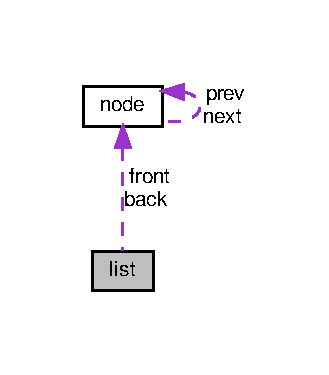
\includegraphics[width=158pt]{structlist__coll__graph}
\end{center}
\end{figure}
\subsection*{Public Attributes}
\begin{DoxyCompactItemize}
\item 
\mbox{\Hypertarget{structlist_a3b03adad0c0429bae9493667ff366dc2}\label{structlist_a3b03adad0c0429bae9493667ff366dc2}} 
int {\bfseries size}
\item 
\mbox{\Hypertarget{structlist_ab5edf0018b269f7eae3d7100ddcea049}\label{structlist_ab5edf0018b269f7eae3d7100ddcea049}} 
\hyperlink{structnode}{node} $\ast$ {\bfseries front}
\item 
\mbox{\Hypertarget{structlist_a92ca5a25484052f219cddb80380a3013}\label{structlist_a92ca5a25484052f219cddb80380a3013}} 
\hyperlink{structnode}{node} $\ast$ {\bfseries back}
\end{DoxyCompactItemize}


The documentation for this struct was generated from the following file\+:\begin{DoxyCompactItemize}
\item 
darknet\+\_\+ros/darknet/include/darknet.\+h\end{DoxyCompactItemize}

\hypertarget{structload__args}{}\section{load\+\_\+args Struct Reference}
\label{structload__args}\index{load\+\_\+args@{load\+\_\+args}}


Collaboration diagram for load\+\_\+args\+:
\nopagebreak
\begin{figure}[H]
\begin{center}
\leavevmode
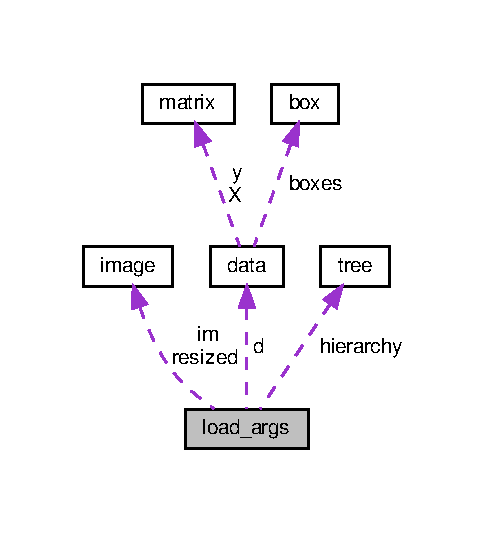
\includegraphics[width=234pt]{structload__args__coll__graph}
\end{center}
\end{figure}
\subsection*{Public Attributes}
\begin{DoxyCompactItemize}
\item 
\mbox{\Hypertarget{structload__args_a3f6b3f3ef9406ab124550bc8166f2dcd}\label{structload__args_a3f6b3f3ef9406ab124550bc8166f2dcd}} 
int {\bfseries threads}
\item 
\mbox{\Hypertarget{structload__args_aadcafc7eb67b2a86a1a7a6ff2ab80a94}\label{structload__args_aadcafc7eb67b2a86a1a7a6ff2ab80a94}} 
char $\ast$$\ast$ {\bfseries paths}
\item 
\mbox{\Hypertarget{structload__args_a2fe0df26f167df4807c7fb67bf835813}\label{structload__args_a2fe0df26f167df4807c7fb67bf835813}} 
char $\ast$ {\bfseries path}
\item 
\mbox{\Hypertarget{structload__args_a46de5db87a3c8c05130d5b23a2cdea2f}\label{structload__args_a46de5db87a3c8c05130d5b23a2cdea2f}} 
int {\bfseries n}
\item 
\mbox{\Hypertarget{structload__args_aca89fa6ea8f11383062a905539477001}\label{structload__args_aca89fa6ea8f11383062a905539477001}} 
int {\bfseries m}
\item 
\mbox{\Hypertarget{structload__args_a66b04c5770c0b451fa14a4a87258be9d}\label{structload__args_a66b04c5770c0b451fa14a4a87258be9d}} 
char $\ast$$\ast$ {\bfseries labels}
\item 
\mbox{\Hypertarget{structload__args_a9cc50b164512ec4db097288e9d569729}\label{structload__args_a9cc50b164512ec4db097288e9d569729}} 
int {\bfseries h}
\item 
\mbox{\Hypertarget{structload__args_a936232a911399499924e00ba80ad16bf}\label{structload__args_a936232a911399499924e00ba80ad16bf}} 
int {\bfseries w}
\item 
\mbox{\Hypertarget{structload__args_aac906990c64be46d44ca7c9895eca6ec}\label{structload__args_aac906990c64be46d44ca7c9895eca6ec}} 
int {\bfseries out\+\_\+w}
\item 
\mbox{\Hypertarget{structload__args_aebbded43f56f35f190cd93501cfb8fa3}\label{structload__args_aebbded43f56f35f190cd93501cfb8fa3}} 
int {\bfseries out\+\_\+h}
\item 
\mbox{\Hypertarget{structload__args_a2a9063dbc5416dc01971bec6a3179a80}\label{structload__args_a2a9063dbc5416dc01971bec6a3179a80}} 
int {\bfseries nh}
\item 
\mbox{\Hypertarget{structload__args_a46bfaa805648b12918b2fff4c66940c7}\label{structload__args_a46bfaa805648b12918b2fff4c66940c7}} 
int {\bfseries nw}
\item 
\mbox{\Hypertarget{structload__args_ac8bdb2525a537b886829037122651101}\label{structload__args_ac8bdb2525a537b886829037122651101}} 
int {\bfseries num\+\_\+boxes}
\item 
\mbox{\Hypertarget{structload__args_a1dceb8bb209570cf9dd9fd5de36f206d}\label{structload__args_a1dceb8bb209570cf9dd9fd5de36f206d}} 
int {\bfseries min}
\item 
\mbox{\Hypertarget{structload__args_a7f5319b3ca7889ed85ac8cc60de8a40d}\label{structload__args_a7f5319b3ca7889ed85ac8cc60de8a40d}} 
int {\bfseries max}
\item 
\mbox{\Hypertarget{structload__args_a57fbd5eb4f1b223ad19b5324fa01b184}\label{structload__args_a57fbd5eb4f1b223ad19b5324fa01b184}} 
int {\bfseries size}
\item 
\mbox{\Hypertarget{structload__args_af12ce52f9bf54ea7985cb0e9b9dfaf55}\label{structload__args_af12ce52f9bf54ea7985cb0e9b9dfaf55}} 
int {\bfseries classes}
\item 
\mbox{\Hypertarget{structload__args_a05d8a43c38b9e069a854cc6a7c7625db}\label{structload__args_a05d8a43c38b9e069a854cc6a7c7625db}} 
int {\bfseries background}
\item 
\mbox{\Hypertarget{structload__args_a27932099db4ddca9b7ca717f92891a44}\label{structload__args_a27932099db4ddca9b7ca717f92891a44}} 
int {\bfseries scale}
\item 
\mbox{\Hypertarget{structload__args_a84a09ba4d910b1129e92dd91fa01d6f0}\label{structload__args_a84a09ba4d910b1129e92dd91fa01d6f0}} 
int {\bfseries center}
\item 
\mbox{\Hypertarget{structload__args_a8db147261d62a355ba735d96f99ada43}\label{structload__args_a8db147261d62a355ba735d96f99ada43}} 
int {\bfseries coords}
\item 
\mbox{\Hypertarget{structload__args_ad446757635db989216a02b331d254906}\label{structload__args_ad446757635db989216a02b331d254906}} 
float {\bfseries jitter}
\item 
\mbox{\Hypertarget{structload__args_a6cc2a92701869043348a92cb810edbbd}\label{structload__args_a6cc2a92701869043348a92cb810edbbd}} 
float {\bfseries angle}
\item 
\mbox{\Hypertarget{structload__args_a0077414b1db970d5eecfc2c756fc328b}\label{structload__args_a0077414b1db970d5eecfc2c756fc328b}} 
float {\bfseries aspect}
\item 
\mbox{\Hypertarget{structload__args_ad478a463de03972022a6c6f89c7c4912}\label{structload__args_ad478a463de03972022a6c6f89c7c4912}} 
float {\bfseries saturation}
\item 
\mbox{\Hypertarget{structload__args_a3db966b80533d8c5003372710f9e8632}\label{structload__args_a3db966b80533d8c5003372710f9e8632}} 
float {\bfseries exposure}
\item 
\mbox{\Hypertarget{structload__args_a37e3681f1edc871b1e15432f08d00114}\label{structload__args_a37e3681f1edc871b1e15432f08d00114}} 
float {\bfseries hue}
\item 
\mbox{\Hypertarget{structload__args_a0b1c4f762d67a0f0cbcc1241cfa5463d}\label{structload__args_a0b1c4f762d67a0f0cbcc1241cfa5463d}} 
\hyperlink{structdata}{data} $\ast$ {\bfseries d}
\item 
\mbox{\Hypertarget{structload__args_ac821b75a2e615c801b67a73911dd0134}\label{structload__args_ac821b75a2e615c801b67a73911dd0134}} 
\hyperlink{structimage}{image} $\ast$ {\bfseries im}
\item 
\mbox{\Hypertarget{structload__args_aa9dc3e3e93a6031df60420a5cb36c508}\label{structload__args_aa9dc3e3e93a6031df60420a5cb36c508}} 
\hyperlink{structimage}{image} $\ast$ {\bfseries resized}
\item 
\mbox{\Hypertarget{structload__args_a281729b932cef85bb4e2a88e1133518d}\label{structload__args_a281729b932cef85bb4e2a88e1133518d}} 
data\+\_\+type {\bfseries type}
\item 
\mbox{\Hypertarget{structload__args_a2c1866cf8b94474f3f8416a1e0f0cf91}\label{structload__args_a2c1866cf8b94474f3f8416a1e0f0cf91}} 
\hyperlink{structtree}{tree} $\ast$ {\bfseries hierarchy}
\end{DoxyCompactItemize}


The documentation for this struct was generated from the following file\+:\begin{DoxyCompactItemize}
\item 
darknet\+\_\+ros/darknet/include/darknet.\+h\end{DoxyCompactItemize}

\hypertarget{structmatrix}{}\section{matrix Struct Reference}
\label{structmatrix}\index{matrix@{matrix}}
\subsection*{Public Attributes}
\begin{DoxyCompactItemize}
\item 
\mbox{\Hypertarget{structmatrix_af83737a5597214de0458c5535a787143}\label{structmatrix_af83737a5597214de0458c5535a787143}} 
int {\bfseries rows}
\item 
\mbox{\Hypertarget{structmatrix_a8a250fb537afd000561485dd88281356}\label{structmatrix_a8a250fb537afd000561485dd88281356}} 
int {\bfseries cols}
\item 
\mbox{\Hypertarget{structmatrix_ac06cdc346e87ea5cb4e4ae1a9b91d61f}\label{structmatrix_ac06cdc346e87ea5cb4e4ae1a9b91d61f}} 
float $\ast$$\ast$ {\bfseries vals}
\end{DoxyCompactItemize}


The documentation for this struct was generated from the following file\+:\begin{DoxyCompactItemize}
\item 
darknet\+\_\+ros/darknet/include/darknet.\+h\end{DoxyCompactItemize}

\hypertarget{structmetadata}{}\section{metadata Struct Reference}
\label{structmetadata}\index{metadata@{metadata}}
\subsection*{Public Attributes}
\begin{DoxyCompactItemize}
\item 
\mbox{\Hypertarget{structmetadata_a79e09a60e76b3658018e342933715f69}\label{structmetadata_a79e09a60e76b3658018e342933715f69}} 
int {\bfseries classes}
\item 
\mbox{\Hypertarget{structmetadata_aee443b3a2259ad9031259d20ddf79086}\label{structmetadata_aee443b3a2259ad9031259d20ddf79086}} 
char $\ast$$\ast$ {\bfseries names}
\end{DoxyCompactItemize}


The documentation for this struct was generated from the following file\+:\begin{DoxyCompactItemize}
\item 
darknet\+\_\+ros/darknet/include/darknet.\+h\end{DoxyCompactItemize}

\hypertarget{classcleanup_1_1_navigation}{}\section{cleanup\+:\+:Navigation Class Reference}
\label{classcleanup_1_1_navigation}\index{cleanup\+::\+Navigation@{cleanup\+::\+Navigation}}


Implementation for navigation routines in R\+OS to command a turtlebot rover.  




{\ttfamily \#include $<$navigation.\+h$>$}

\subsection*{Public Member Functions}
\begin{DoxyCompactItemize}
\item 
\mbox{\Hypertarget{classcleanup_1_1_navigation_ae4f3e6facf6e48e4286cf751a8be6fb1}\label{classcleanup_1_1_navigation_ae4f3e6facf6e48e4286cf751a8be6fb1}} 
\hyperlink{classcleanup_1_1_navigation_ae4f3e6facf6e48e4286cf751a8be6fb1}{Navigation} ()
\begin{DoxyCompactList}\small\item\em Constructor. \end{DoxyCompactList}\item 
\mbox{\Hypertarget{classcleanup_1_1_navigation_ab6e850bcac11ad0a06f371053844cddc}\label{classcleanup_1_1_navigation_ab6e850bcac11ad0a06f371053844cddc}} 
\hyperlink{classcleanup_1_1_navigation_ab6e850bcac11ad0a06f371053844cddc}{$\sim$\+Navigation} ()
\begin{DoxyCompactList}\small\item\em Destructor. \end{DoxyCompactList}\item 
void \hyperlink{classcleanup_1_1_navigation_a4990de9c7d80e4bd64dbb40f7bac596e}{explore\+Loop} ()
\begin{DoxyCompactList}\small\item\em Explore the given area, avoiding obstacles. \end{DoxyCompactList}\item 
\mbox{\Hypertarget{classcleanup_1_1_navigation_aa95c5e9bef0d4780c828ee5952964f8f}\label{classcleanup_1_1_navigation_aa95c5e9bef0d4780c828ee5952964f8f}} 
void \hyperlink{classcleanup_1_1_navigation_aa95c5e9bef0d4780c828ee5952964f8f}{stop} ()
\begin{DoxyCompactList}\small\item\em Stop any running threads and navigation goals. \end{DoxyCompactList}\item 
geometry\+\_\+msgs\+::\+Pose \hyperlink{classcleanup_1_1_navigation_a4b39246f07e511da75444ca2ed655326}{get\+Robot\+Pose} ()
\begin{DoxyCompactList}\small\item\em Get current robot position. \end{DoxyCompactList}\item 
\mbox{\Hypertarget{classcleanup_1_1_navigation_abde0f634a0a8bee3603c16ae921c772a}\label{classcleanup_1_1_navigation_abde0f634a0a8bee3603c16ae921c772a}} 
int \hyperlink{classcleanup_1_1_navigation_abde0f634a0a8bee3603c16ae921c772a}{get\+Curr\+Nav\+Mode} ()
\begin{DoxyCompactList}\small\item\em Get integer related to current Set\+Mode\+Goal. \end{DoxyCompactList}\end{DoxyCompactItemize}


\subsection{Detailed Description}
Implementation for navigation routines in R\+OS to command a turtlebot rover. 

\subsection{Member Function Documentation}
\mbox{\Hypertarget{classcleanup_1_1_navigation_a4990de9c7d80e4bd64dbb40f7bac596e}\label{classcleanup_1_1_navigation_a4990de9c7d80e4bd64dbb40f7bac596e}} 
\index{cleanup\+::\+Navigation@{cleanup\+::\+Navigation}!explore\+Loop@{explore\+Loop}}
\index{explore\+Loop@{explore\+Loop}!cleanup\+::\+Navigation@{cleanup\+::\+Navigation}}
\subsubsection{\texorpdfstring{explore\+Loop()}{exploreLoop()}}
{\footnotesize\ttfamily void cleanup\+::\+Navigation\+::explore\+Loop (\begin{DoxyParamCaption}{ }\end{DoxyParamCaption})}



Explore the given area, avoiding obstacles. 

The basic implementation is just to move in straight lines until an obstacle is encountered, then rotate until the way ahead is clear.

This calls \hyperlink{classcleanup_1_1_navigation_aa95c5e9bef0d4780c828ee5952964f8f}{stop()} implictly. \mbox{\Hypertarget{classcleanup_1_1_navigation_a4b39246f07e511da75444ca2ed655326}\label{classcleanup_1_1_navigation_a4b39246f07e511da75444ca2ed655326}} 
\index{cleanup\+::\+Navigation@{cleanup\+::\+Navigation}!get\+Robot\+Pose@{get\+Robot\+Pose}}
\index{get\+Robot\+Pose@{get\+Robot\+Pose}!cleanup\+::\+Navigation@{cleanup\+::\+Navigation}}
\subsubsection{\texorpdfstring{get\+Robot\+Pose()}{getRobotPose()}}
{\footnotesize\ttfamily geometry\+\_\+msgs\+::\+Pose cleanup\+::\+Navigation\+::get\+Robot\+Pose (\begin{DoxyParamCaption}{ }\end{DoxyParamCaption})}



Get current robot position. 

\begin{DoxyReturn}{Returns}
Current pose of robot (world position, world rotation) 
\end{DoxyReturn}


The documentation for this class was generated from the following files\+:\begin{DoxyCompactItemize}
\item 
navigation/include/navigation/\hyperlink{navigation_8h}{navigation.\+h}\item 
navigation/src/\hyperlink{navigation_8cpp}{navigation.\+cpp}\end{DoxyCompactItemize}

\hypertarget{structnetwork}{}\section{network Struct Reference}
\label{structnetwork}\index{network@{network}}


Collaboration diagram for network\+:\nopagebreak
\begin{figure}[H]
\begin{center}
\leavevmode
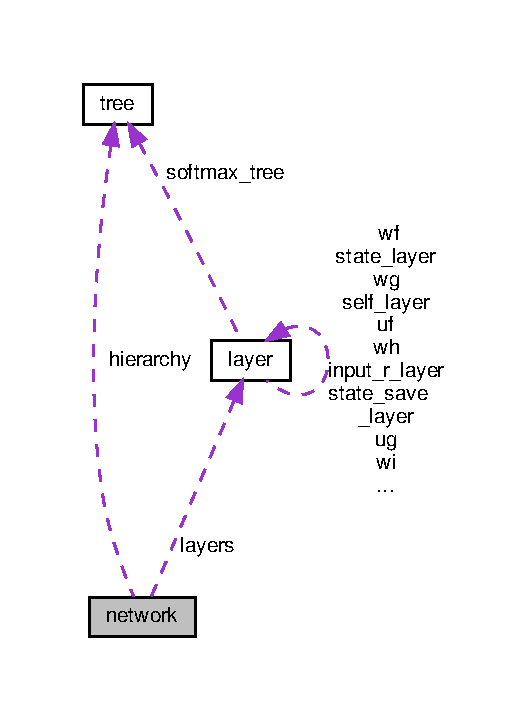
\includegraphics[width=254pt]{structnetwork__coll__graph}
\end{center}
\end{figure}
\subsection*{Public Attributes}
\begin{DoxyCompactItemize}
\item 
\mbox{\Hypertarget{structnetwork_a1c7625720955322d05924a075d013877}\label{structnetwork_a1c7625720955322d05924a075d013877}} 
int {\bfseries n}
\item 
\mbox{\Hypertarget{structnetwork_a04f448f3f8c3f1314e2b23b429bec827}\label{structnetwork_a04f448f3f8c3f1314e2b23b429bec827}} 
int {\bfseries batch}
\item 
\mbox{\Hypertarget{structnetwork_aaa4dc3920fc905e52573172d45fccd45}\label{structnetwork_aaa4dc3920fc905e52573172d45fccd45}} 
size\+\_\+t $\ast$ {\bfseries seen}
\item 
\mbox{\Hypertarget{structnetwork_a185b52d74237f3cd32d2d0186d2d2f5b}\label{structnetwork_a185b52d74237f3cd32d2d0186d2d2f5b}} 
int $\ast$ {\bfseries t}
\item 
\mbox{\Hypertarget{structnetwork_a7b16b097d1814258e82b58d663692875}\label{structnetwork_a7b16b097d1814258e82b58d663692875}} 
float {\bfseries epoch}
\item 
\mbox{\Hypertarget{structnetwork_ab30643da07e0f787ee0cd2058cd41a6e}\label{structnetwork_ab30643da07e0f787ee0cd2058cd41a6e}} 
int {\bfseries subdivisions}
\item 
\mbox{\Hypertarget{structnetwork_a9770423f88b722bafc9d1fd3c6091d75}\label{structnetwork_a9770423f88b722bafc9d1fd3c6091d75}} 
\hyperlink{structlayer}{layer} $\ast$ {\bfseries layers}
\item 
\mbox{\Hypertarget{structnetwork_a274dce0db2d5175992eb3b273ab09df7}\label{structnetwork_a274dce0db2d5175992eb3b273ab09df7}} 
float $\ast$ {\bfseries output}
\item 
\mbox{\Hypertarget{structnetwork_a78121635a0f0c3a1d9991390b4325dc3}\label{structnetwork_a78121635a0f0c3a1d9991390b4325dc3}} 
learning\+\_\+rate\+\_\+policy {\bfseries policy}
\item 
\mbox{\Hypertarget{structnetwork_a978d3e339536cd6bea2270d49d93c35a}\label{structnetwork_a978d3e339536cd6bea2270d49d93c35a}} 
float {\bfseries learning\+\_\+rate}
\item 
\mbox{\Hypertarget{structnetwork_a495c60ef821ca0ade1c42907c8bc90bf}\label{structnetwork_a495c60ef821ca0ade1c42907c8bc90bf}} 
float {\bfseries momentum}
\item 
\mbox{\Hypertarget{structnetwork_a9afd53b100d35dc162e48118ef4f7eea}\label{structnetwork_a9afd53b100d35dc162e48118ef4f7eea}} 
float {\bfseries decay}
\item 
\mbox{\Hypertarget{structnetwork_a5460d67e44c0877ca016ed12925788fe}\label{structnetwork_a5460d67e44c0877ca016ed12925788fe}} 
float {\bfseries gamma}
\item 
\mbox{\Hypertarget{structnetwork_a0d9e7af8dde42e28a7fdb0e685b2f23b}\label{structnetwork_a0d9e7af8dde42e28a7fdb0e685b2f23b}} 
float {\bfseries scale}
\item 
\mbox{\Hypertarget{structnetwork_ae38f864b7b9966c38f1882f468131eda}\label{structnetwork_ae38f864b7b9966c38f1882f468131eda}} 
float {\bfseries power}
\item 
\mbox{\Hypertarget{structnetwork_abaf83235b5968fb68a2dc9215cc67c8c}\label{structnetwork_abaf83235b5968fb68a2dc9215cc67c8c}} 
int {\bfseries time\+\_\+steps}
\item 
\mbox{\Hypertarget{structnetwork_a9ed08472400f140c49ecac3ecd1def87}\label{structnetwork_a9ed08472400f140c49ecac3ecd1def87}} 
int {\bfseries step}
\item 
\mbox{\Hypertarget{structnetwork_a163b931990a5ac8f456884405de2192b}\label{structnetwork_a163b931990a5ac8f456884405de2192b}} 
int {\bfseries max\+\_\+batches}
\item 
\mbox{\Hypertarget{structnetwork_a64c1fa0153559f530cc815fb6b8a95c8}\label{structnetwork_a64c1fa0153559f530cc815fb6b8a95c8}} 
float $\ast$ {\bfseries scales}
\item 
\mbox{\Hypertarget{structnetwork_a48fb87937b7ff22cf01875d8d5807cc2}\label{structnetwork_a48fb87937b7ff22cf01875d8d5807cc2}} 
int $\ast$ {\bfseries steps}
\item 
\mbox{\Hypertarget{structnetwork_a6e656092c18afdc2bcb72f87d0ed2547}\label{structnetwork_a6e656092c18afdc2bcb72f87d0ed2547}} 
int {\bfseries num\+\_\+steps}
\item 
\mbox{\Hypertarget{structnetwork_a1e0395e7cbcd9cd93d5c8621bb1a38aa}\label{structnetwork_a1e0395e7cbcd9cd93d5c8621bb1a38aa}} 
int {\bfseries burn\+\_\+in}
\item 
\mbox{\Hypertarget{structnetwork_a7274661135ee8efe567aef0e9c0e40f9}\label{structnetwork_a7274661135ee8efe567aef0e9c0e40f9}} 
int {\bfseries adam}
\item 
\mbox{\Hypertarget{structnetwork_a6c56d5eccebbfd39c085766b94cd36b7}\label{structnetwork_a6c56d5eccebbfd39c085766b94cd36b7}} 
float {\bfseries B1}
\item 
\mbox{\Hypertarget{structnetwork_a42ea583b98356e06dca647bf95520e5c}\label{structnetwork_a42ea583b98356e06dca647bf95520e5c}} 
float {\bfseries B2}
\item 
\mbox{\Hypertarget{structnetwork_a13a150c894a1f34f08b7f8dff7808ea7}\label{structnetwork_a13a150c894a1f34f08b7f8dff7808ea7}} 
float {\bfseries eps}
\item 
\mbox{\Hypertarget{structnetwork_a529a36505548232d049abcb84fdcf389}\label{structnetwork_a529a36505548232d049abcb84fdcf389}} 
int {\bfseries inputs}
\item 
\mbox{\Hypertarget{structnetwork_a5268de11127a02d86e6f517cf3b3acc9}\label{structnetwork_a5268de11127a02d86e6f517cf3b3acc9}} 
int {\bfseries outputs}
\item 
\mbox{\Hypertarget{structnetwork_a794927f8c4d44cd8e85ff39e0d4c9939}\label{structnetwork_a794927f8c4d44cd8e85ff39e0d4c9939}} 
int {\bfseries truths}
\item 
\mbox{\Hypertarget{structnetwork_a6769bc5e23225cecf0a46eedba29719a}\label{structnetwork_a6769bc5e23225cecf0a46eedba29719a}} 
int {\bfseries notruth}
\item 
\mbox{\Hypertarget{structnetwork_a0e57f4230f8ecb07bba0c97cf8f045c7}\label{structnetwork_a0e57f4230f8ecb07bba0c97cf8f045c7}} 
int {\bfseries h}
\item 
\mbox{\Hypertarget{structnetwork_a944b83cb20da2454c6092e07b9a1d3e9}\label{structnetwork_a944b83cb20da2454c6092e07b9a1d3e9}} 
int {\bfseries w}
\item 
\mbox{\Hypertarget{structnetwork_a05014921b926874b8a362aa83d98283a}\label{structnetwork_a05014921b926874b8a362aa83d98283a}} 
int {\bfseries c}
\item 
\mbox{\Hypertarget{structnetwork_af98abf1cccd7bfee97b9f7eae752687c}\label{structnetwork_af98abf1cccd7bfee97b9f7eae752687c}} 
int {\bfseries max\+\_\+crop}
\item 
\mbox{\Hypertarget{structnetwork_a9e52bfae3a850150ed2e32c10ab11bec}\label{structnetwork_a9e52bfae3a850150ed2e32c10ab11bec}} 
int {\bfseries min\+\_\+crop}
\item 
\mbox{\Hypertarget{structnetwork_a181329911f37d2d5adce2290683a9897}\label{structnetwork_a181329911f37d2d5adce2290683a9897}} 
float {\bfseries max\+\_\+ratio}
\item 
\mbox{\Hypertarget{structnetwork_a395ccde63912c9272f91ee6c9af14784}\label{structnetwork_a395ccde63912c9272f91ee6c9af14784}} 
float {\bfseries min\+\_\+ratio}
\item 
\mbox{\Hypertarget{structnetwork_a87bf27881ed88606fae1b80f9049e4ca}\label{structnetwork_a87bf27881ed88606fae1b80f9049e4ca}} 
int {\bfseries center}
\item 
\mbox{\Hypertarget{structnetwork_abe286813534c121ee16da09c258eaf2e}\label{structnetwork_abe286813534c121ee16da09c258eaf2e}} 
float {\bfseries angle}
\item 
\mbox{\Hypertarget{structnetwork_acaa88cf6c30100edff5dc061bfb226bb}\label{structnetwork_acaa88cf6c30100edff5dc061bfb226bb}} 
float {\bfseries aspect}
\item 
\mbox{\Hypertarget{structnetwork_a609572db2c14c55c6c261844cb33fa12}\label{structnetwork_a609572db2c14c55c6c261844cb33fa12}} 
float {\bfseries exposure}
\item 
\mbox{\Hypertarget{structnetwork_a9bbb55144a6eca464fbc122f97bf1af8}\label{structnetwork_a9bbb55144a6eca464fbc122f97bf1af8}} 
float {\bfseries saturation}
\item 
\mbox{\Hypertarget{structnetwork_ae38058a4e1ad0a334026ecbe01f101f4}\label{structnetwork_ae38058a4e1ad0a334026ecbe01f101f4}} 
float {\bfseries hue}
\item 
\mbox{\Hypertarget{structnetwork_a89dfdaa6178f338c250d7b6631476fa1}\label{structnetwork_a89dfdaa6178f338c250d7b6631476fa1}} 
int {\bfseries random}
\item 
\mbox{\Hypertarget{structnetwork_a8ba8b1354e8d018ac74920eb0cd882e8}\label{structnetwork_a8ba8b1354e8d018ac74920eb0cd882e8}} 
int {\bfseries gpu\+\_\+index}
\item 
\mbox{\Hypertarget{structnetwork_a36d6158f07498646e400bf6f7e20a705}\label{structnetwork_a36d6158f07498646e400bf6f7e20a705}} 
\hyperlink{structtree}{tree} $\ast$ {\bfseries hierarchy}
\item 
\mbox{\Hypertarget{structnetwork_a8f391155a3ceb60caf07d0ee6c6a93f2}\label{structnetwork_a8f391155a3ceb60caf07d0ee6c6a93f2}} 
float $\ast$ {\bfseries input}
\item 
\mbox{\Hypertarget{structnetwork_a1453c2cf9a735bde55a281d698797a05}\label{structnetwork_a1453c2cf9a735bde55a281d698797a05}} 
float $\ast$ {\bfseries truth}
\item 
\mbox{\Hypertarget{structnetwork_a7787a7dde0eea2d91b208c23cdba6286}\label{structnetwork_a7787a7dde0eea2d91b208c23cdba6286}} 
float $\ast$ {\bfseries delta}
\item 
\mbox{\Hypertarget{structnetwork_a624719738b94a1d55de651f5dac16b79}\label{structnetwork_a624719738b94a1d55de651f5dac16b79}} 
float $\ast$ {\bfseries workspace}
\item 
\mbox{\Hypertarget{structnetwork_a32e7b55fe8dfa07391b6cdce17b4a2c1}\label{structnetwork_a32e7b55fe8dfa07391b6cdce17b4a2c1}} 
int {\bfseries train}
\item 
\mbox{\Hypertarget{structnetwork_a67a4b2779829a2891b1e3194b4910334}\label{structnetwork_a67a4b2779829a2891b1e3194b4910334}} 
int {\bfseries index}
\item 
\mbox{\Hypertarget{structnetwork_ac80b4b4eeda5cf4cc4af5c2173d0ad31}\label{structnetwork_ac80b4b4eeda5cf4cc4af5c2173d0ad31}} 
float $\ast$ {\bfseries cost}
\item 
\mbox{\Hypertarget{structnetwork_ac04afd1b20edc7f8734cf2eabe4b57f0}\label{structnetwork_ac04afd1b20edc7f8734cf2eabe4b57f0}} 
float {\bfseries clip}
\end{DoxyCompactItemize}


The documentation for this struct was generated from the following file\+:\begin{DoxyCompactItemize}
\item 
darknet\+\_\+ros/darknet/include/darknet.\+h\end{DoxyCompactItemize}

\hypertarget{structnode}{}\section{node Struct Reference}
\label{structnode}\index{node@{node}}


Collaboration diagram for node\+:\nopagebreak
\begin{figure}[H]
\begin{center}
\leavevmode
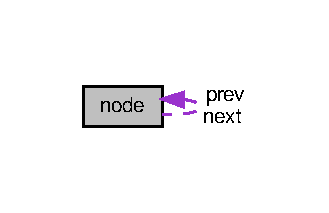
\includegraphics[width=158pt]{structnode__coll__graph}
\end{center}
\end{figure}
\subsection*{Public Attributes}
\begin{DoxyCompactItemize}
\item 
\mbox{\Hypertarget{structnode_a3866f55c05d50265b730d8cdeec0a1f8}\label{structnode_a3866f55c05d50265b730d8cdeec0a1f8}} 
void $\ast$ {\bfseries val}
\item 
\mbox{\Hypertarget{structnode_aa3e8aa83f864292b5a01210f4453fcc0}\label{structnode_aa3e8aa83f864292b5a01210f4453fcc0}} 
struct \hyperlink{structnode}{node} $\ast$ {\bfseries next}
\item 
\mbox{\Hypertarget{structnode_a7ee3d227c728ce18a86e43ebc301046e}\label{structnode_a7ee3d227c728ce18a86e43ebc301046e}} 
struct \hyperlink{structnode}{node} $\ast$ {\bfseries prev}
\end{DoxyCompactItemize}


The documentation for this struct was generated from the following file\+:\begin{DoxyCompactItemize}
\item 
darknet\+\_\+ros/darknet/include/darknet.\+h\end{DoxyCompactItemize}

\hypertarget{classcleanup_1_1_perception}{}\section{cleanup\+:\+:Perception Class Reference}
\label{classcleanup_1_1_perception}\index{cleanup\+::\+Perception@{cleanup\+::\+Perception}}
\subsection*{Public Member Functions}
\begin{DoxyCompactItemize}
\item 
std\+::vector$<$ int $>$ \hyperlink{classcleanup_1_1_perception_a8928e5e59df7651a833505aec0cd7e4f}{detect\+Objects} ()
\begin{DoxyCompactList}\small\item\em Function to store the detected objects. \end{DoxyCompactList}\item 
geometry\+\_\+msgs\+::\+Pose\+Stamped \hyperlink{classcleanup_1_1_perception_a602ed7efc2ca9d418daa2aed25f4e3ba}{get\+Object\+Pose} ()
\begin{DoxyCompactList}\small\item\em Function to known the object\textquotesingle{}s pose. \end{DoxyCompactList}\item 
\mbox{\Hypertarget{classcleanup_1_1_perception_aef837fda07b38e8746776d35925e36e4}\label{classcleanup_1_1_perception_aef837fda07b38e8746776d35925e36e4}} 
void \hyperlink{classcleanup_1_1_perception_aef837fda07b38e8746776d35925e36e4}{image\+Callback} ()
\begin{DoxyCompactList}\small\item\em Image callback Function. \end{DoxyCompactList}\item 
\mbox{\Hypertarget{classcleanup_1_1_perception_aa2406cbc9ac17c40c5bcdfc9b98f369d}\label{classcleanup_1_1_perception_aa2406cbc9ac17c40c5bcdfc9b98f369d}} 
void \hyperlink{classcleanup_1_1_perception_aa2406cbc9ac17c40c5bcdfc9b98f369d}{run\+Vision\+Algo} ()
\begin{DoxyCompactList}\small\item\em Robust vision algorithm to detect objects and obstacles. \end{DoxyCompactList}\end{DoxyCompactItemize}


\subsection{Member Function Documentation}
\mbox{\Hypertarget{classcleanup_1_1_perception_a8928e5e59df7651a833505aec0cd7e4f}\label{classcleanup_1_1_perception_a8928e5e59df7651a833505aec0cd7e4f}} 
\index{cleanup\+::\+Perception@{cleanup\+::\+Perception}!detect\+Objects@{detect\+Objects}}
\index{detect\+Objects@{detect\+Objects}!cleanup\+::\+Perception@{cleanup\+::\+Perception}}
\subsubsection{\texorpdfstring{detect\+Objects()}{detectObjects()}}
{\footnotesize\ttfamily std\+::vector$<$ int $>$ cleanup\+::\+Perception\+::detect\+Objects (\begin{DoxyParamCaption}{ }\end{DoxyParamCaption})}



Function to store the detected objects. 

\begin{DoxyReturn}{Returns}
vector of ids 
\end{DoxyReturn}
\mbox{\Hypertarget{classcleanup_1_1_perception_a602ed7efc2ca9d418daa2aed25f4e3ba}\label{classcleanup_1_1_perception_a602ed7efc2ca9d418daa2aed25f4e3ba}} 
\index{cleanup\+::\+Perception@{cleanup\+::\+Perception}!get\+Object\+Pose@{get\+Object\+Pose}}
\index{get\+Object\+Pose@{get\+Object\+Pose}!cleanup\+::\+Perception@{cleanup\+::\+Perception}}
\subsubsection{\texorpdfstring{get\+Object\+Pose()}{getObjectPose()}}
{\footnotesize\ttfamily geometry\+\_\+msgs\+::\+Pose\+Stamped cleanup\+::\+Perception\+::get\+Object\+Pose (\begin{DoxyParamCaption}{ }\end{DoxyParamCaption})}



Function to known the object\textquotesingle{}s pose. 

\begin{DoxyReturn}{Returns}
The object pose. 
\end{DoxyReturn}


The documentation for this class was generated from the following files\+:\begin{DoxyCompactItemize}
\item 
perception/include/perception/perception.\+h\item 
perception/src/perception.\+cpp\end{DoxyCompactItemize}

\hypertarget{structstbi__io__callbacks}{}\section{stbi\+\_\+io\+\_\+callbacks Struct Reference}
\label{structstbi__io__callbacks}\index{stbi\+\_\+io\+\_\+callbacks@{stbi\+\_\+io\+\_\+callbacks}}
\subsection*{Public Attributes}
\begin{DoxyCompactItemize}
\item 
\mbox{\Hypertarget{structstbi__io__callbacks_a623e46b3a2a019611601409926283a88}\label{structstbi__io__callbacks_a623e46b3a2a019611601409926283a88}} 
int($\ast$ {\bfseries read} )(void $\ast$user, char $\ast$\hyperlink{structdata}{data}, int size)
\item 
\mbox{\Hypertarget{structstbi__io__callbacks_a257aac5480a90a6c4b8fbe86c1b01068}\label{structstbi__io__callbacks_a257aac5480a90a6c4b8fbe86c1b01068}} 
void($\ast$ {\bfseries skip} )(void $\ast$user, int n)
\item 
\mbox{\Hypertarget{structstbi__io__callbacks_a319639db2f76e715eed7a7a974136832}\label{structstbi__io__callbacks_a319639db2f76e715eed7a7a974136832}} 
int($\ast$ {\bfseries eof} )(void $\ast$user)
\end{DoxyCompactItemize}


The documentation for this struct was generated from the following file\+:\begin{DoxyCompactItemize}
\item 
darknet\+\_\+ros/darknet/src/stb\+\_\+image.\+h\end{DoxyCompactItemize}

\hypertarget{structtree}{}\section{tree Struct Reference}
\label{structtree}\index{tree@{tree}}
\subsection*{Public Attributes}
\begin{DoxyCompactItemize}
\item 
\mbox{\Hypertarget{structtree_a08371bc037edecea4f1632c2185b1ff1}\label{structtree_a08371bc037edecea4f1632c2185b1ff1}} 
int $\ast$ {\bfseries leaf}
\item 
\mbox{\Hypertarget{structtree_a2273fc7497601bfaf9121d1a797453b5}\label{structtree_a2273fc7497601bfaf9121d1a797453b5}} 
int {\bfseries n}
\item 
\mbox{\Hypertarget{structtree_a77b1eb5cb07b504420034ed006f75cb5}\label{structtree_a77b1eb5cb07b504420034ed006f75cb5}} 
int $\ast$ {\bfseries parent}
\item 
\mbox{\Hypertarget{structtree_ac33525f8c2ea9df09aa39e4e5f0f46b0}\label{structtree_ac33525f8c2ea9df09aa39e4e5f0f46b0}} 
int $\ast$ {\bfseries child}
\item 
\mbox{\Hypertarget{structtree_a3accabb15b1b96d0f81e40341e55cc20}\label{structtree_a3accabb15b1b96d0f81e40341e55cc20}} 
int $\ast$ {\bfseries group}
\item 
\mbox{\Hypertarget{structtree_aef62d17752842a143625d7313073c068}\label{structtree_aef62d17752842a143625d7313073c068}} 
char $\ast$$\ast$ {\bfseries name}
\item 
\mbox{\Hypertarget{structtree_ab4d92fc866330ea5e427d6b5b8075604}\label{structtree_ab4d92fc866330ea5e427d6b5b8075604}} 
int {\bfseries groups}
\item 
\mbox{\Hypertarget{structtree_a4b84be443f42bcf6cc16fd9d3fa1f326}\label{structtree_a4b84be443f42bcf6cc16fd9d3fa1f326}} 
int $\ast$ {\bfseries group\+\_\+size}
\item 
\mbox{\Hypertarget{structtree_a349dec53fea0efa2e19de49785a2f0ff}\label{structtree_a349dec53fea0efa2e19de49785a2f0ff}} 
int $\ast$ {\bfseries group\+\_\+offset}
\end{DoxyCompactItemize}


The documentation for this struct was generated from the following file\+:\begin{DoxyCompactItemize}
\item 
darknet\+\_\+ros/darknet/include/darknet.\+h\end{DoxyCompactItemize}

\hypertarget{structupdate__args}{}\section{update\+\_\+args Struct Reference}
\label{structupdate__args}\index{update\+\_\+args@{update\+\_\+args}}
\subsection*{Public Attributes}
\begin{DoxyCompactItemize}
\item 
\mbox{\Hypertarget{structupdate__args_a1accceb722234c5aa3f38cc85c1d7cf7}\label{structupdate__args_a1accceb722234c5aa3f38cc85c1d7cf7}} 
int {\bfseries batch}
\item 
\mbox{\Hypertarget{structupdate__args_a3a0145d580360b2ffae2879af7e68c67}\label{structupdate__args_a3a0145d580360b2ffae2879af7e68c67}} 
float {\bfseries learning\+\_\+rate}
\item 
\mbox{\Hypertarget{structupdate__args_abc35ad880888473f137cb9744e874870}\label{structupdate__args_abc35ad880888473f137cb9744e874870}} 
float {\bfseries momentum}
\item 
\mbox{\Hypertarget{structupdate__args_a9eb5a4b5663dca4b69a13a19da674f19}\label{structupdate__args_a9eb5a4b5663dca4b69a13a19da674f19}} 
float {\bfseries decay}
\item 
\mbox{\Hypertarget{structupdate__args_ab246da6c016ed395f727ab4f12df6e7d}\label{structupdate__args_ab246da6c016ed395f727ab4f12df6e7d}} 
int {\bfseries adam}
\item 
\mbox{\Hypertarget{structupdate__args_a1822b0d844c349135590f3583415faec}\label{structupdate__args_a1822b0d844c349135590f3583415faec}} 
float {\bfseries B1}
\item 
\mbox{\Hypertarget{structupdate__args_ad4542261082ee829820f2d6a750021f6}\label{structupdate__args_ad4542261082ee829820f2d6a750021f6}} 
float {\bfseries B2}
\item 
\mbox{\Hypertarget{structupdate__args_a7a173936c93e7424d77347cfa9ab3f2f}\label{structupdate__args_a7a173936c93e7424d77347cfa9ab3f2f}} 
float {\bfseries eps}
\item 
\mbox{\Hypertarget{structupdate__args_addc09d90e7323fc19a4e04b0612ef10b}\label{structupdate__args_addc09d90e7323fc19a4e04b0612ef10b}} 
int {\bfseries t}
\end{DoxyCompactItemize}


The documentation for this struct was generated from the following file\+:\begin{DoxyCompactItemize}
\item 
darknet\+\_\+ros/darknet/include/darknet.\+h\end{DoxyCompactItemize}

\hypertarget{classcleanup_1_1_user_panel}{}\section{cleanup\+:\+:User\+Panel Class Reference}
\label{classcleanup_1_1_user_panel}\index{cleanup\+::\+User\+Panel@{cleanup\+::\+User\+Panel}}


Implementation for a custom user panel in R\+V\+IZ.  




{\ttfamily \#include $<$user\+\_\+panel.\+h$>$}



Inheritance diagram for cleanup\+:\+:User\+Panel\+:\nopagebreak
\begin{figure}[H]
\begin{center}
\leavevmode
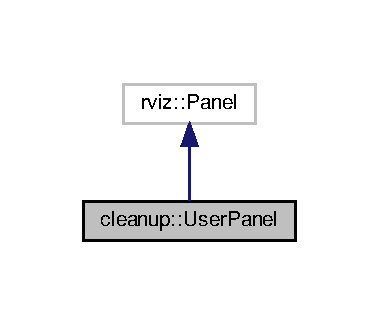
\includegraphics[width=182pt]{classcleanup_1_1_user_panel__inherit__graph}
\end{center}
\end{figure}


Collaboration diagram for cleanup\+:\+:User\+Panel\+:\nopagebreak
\begin{figure}[H]
\begin{center}
\leavevmode
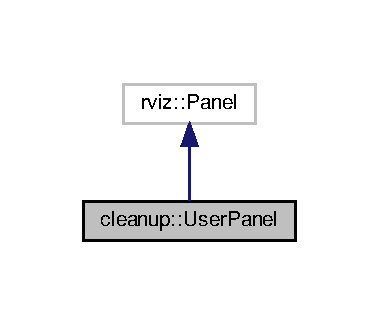
\includegraphics[width=182pt]{classcleanup_1_1_user_panel__coll__graph}
\end{center}
\end{figure}
\subsection*{Public Slots}
\begin{DoxyCompactItemize}
\item 
\mbox{\Hypertarget{classcleanup_1_1_user_panel_a66a9e5c66aea653517d628c8b9ecc854}\label{classcleanup_1_1_user_panel_a66a9e5c66aea653517d628c8b9ecc854}} 
void \hyperlink{classcleanup_1_1_user_panel_a66a9e5c66aea653517d628c8b9ecc854}{explore} ()
\begin{DoxyCompactList}\small\item\em Call Explore function. \end{DoxyCompactList}\item 
\mbox{\Hypertarget{classcleanup_1_1_user_panel_aba5df97a2ea3e7b56eb4df3291103053}\label{classcleanup_1_1_user_panel_aba5df97a2ea3e7b56eb4df3291103053}} 
void \hyperlink{classcleanup_1_1_user_panel_aba5df97a2ea3e7b56eb4df3291103053}{clean} ()
\begin{DoxyCompactList}\small\item\em Call Clean function. \end{DoxyCompactList}\item 
\mbox{\Hypertarget{classcleanup_1_1_user_panel_aebd2aebbe8a8e87ad2d8c7618d286f58}\label{classcleanup_1_1_user_panel_aebd2aebbe8a8e87ad2d8c7618d286f58}} 
void \hyperlink{classcleanup_1_1_user_panel_aebd2aebbe8a8e87ad2d8c7618d286f58}{stop} ()
\begin{DoxyCompactList}\small\item\em Call Stop function. \end{DoxyCompactList}\end{DoxyCompactItemize}
\subsection*{Public Member Functions}
\begin{DoxyCompactItemize}
\item 
\mbox{\Hypertarget{classcleanup_1_1_user_panel_a728e7c90ec9c6e9714c0660615d705fc}\label{classcleanup_1_1_user_panel_a728e7c90ec9c6e9714c0660615d705fc}} 
\hyperlink{classcleanup_1_1_user_panel_a728e7c90ec9c6e9714c0660615d705fc}{User\+Panel} (Q\+Widget $\ast$parent=0)
\begin{DoxyCompactList}\small\item\em Constructor. \end{DoxyCompactList}\end{DoxyCompactItemize}
\subsection*{Protected Member Functions}
\begin{DoxyCompactItemize}
\item 
\mbox{\Hypertarget{classcleanup_1_1_user_panel_a02f7e7b8a4e28ffb92f1acb79087079e}\label{classcleanup_1_1_user_panel_a02f7e7b8a4e28ffb92f1acb79087079e}} 
void {\bfseries send\+Goal} (const std\+::string \&mode)
\end{DoxyCompactItemize}
\subsection*{Protected Attributes}
\begin{DoxyCompactItemize}
\item 
\mbox{\Hypertarget{classcleanup_1_1_user_panel_a718b588057cc72b9edbfc1f9c2f0c084}\label{classcleanup_1_1_user_panel_a718b588057cc72b9edbfc1f9c2f0c084}} 
Q\+Push\+Button $\ast$ {\bfseries explore\+\_\+button\+\_\+}
\item 
\mbox{\Hypertarget{classcleanup_1_1_user_panel_a898a0f77d79438ee266e119303613606}\label{classcleanup_1_1_user_panel_a898a0f77d79438ee266e119303613606}} 
Q\+Push\+Button $\ast$ {\bfseries clean\+\_\+button\+\_\+}
\item 
\mbox{\Hypertarget{classcleanup_1_1_user_panel_a9cb1f405edd75371c1a14a5dcd4fa038}\label{classcleanup_1_1_user_panel_a9cb1f405edd75371c1a14a5dcd4fa038}} 
Q\+Push\+Button $\ast$ {\bfseries stop\+\_\+button\+\_\+}
\item 
\mbox{\Hypertarget{classcleanup_1_1_user_panel_aa4b3efececbc9296c40f180e94dee7c7}\label{classcleanup_1_1_user_panel_aa4b3efececbc9296c40f180e94dee7c7}} 
ros\+::\+Node\+Handle {\bfseries nh\+\_\+}
\item 
\mbox{\Hypertarget{classcleanup_1_1_user_panel_a09cc36d63b054e7dd0a849de9d921be8}\label{classcleanup_1_1_user_panel_a09cc36d63b054e7dd0a849de9d921be8}} 
actionlib\+::\+Simple\+Action\+Client$<$ controller\+::\+Set\+Mode\+Action $>$ {\bfseries client\+\_\+}
\end{DoxyCompactItemize}


\subsection{Detailed Description}
Implementation for a custom user panel in R\+V\+IZ. 

The documentation for this class was generated from the following files\+:\begin{DoxyCompactItemize}
\item 
controller/src/\hyperlink{user__panel_8h}{user\+\_\+panel.\+h}\item 
controller/src/\hyperlink{user__panel_8cpp}{user\+\_\+panel.\+cpp}\end{DoxyCompactItemize}

\chapter{File Documentation}
\hypertarget{controller_8h}{}\section{controller/include/controller/controller.h File Reference}
\label{controller_8h}\index{controller/include/controller/controller.\+h@{controller/include/controller/controller.\+h}}


Header of the Controller class for overall system management.  


{\ttfamily \#include $<$ros/ros.\+h$>$}\newline
{\ttfamily \#include $<$actionlib/server/simple\+\_\+action\+\_\+server.\+h$>$}\newline
{\ttfamily \#include $<$std\+\_\+srvs/\+Trigger.\+h$>$}\newline
{\ttfamily \#include $<$navigation/\+Set\+Pose\+Stamped.\+h$>$}\newline
{\ttfamily \#include $<$controller/\+Set\+Mode\+Action.\+h$>$}\newline
{\ttfamily \#include $<$memory$>$}\newline
Include dependency graph for controller.\+h\+:
\nopagebreak
\begin{figure}[H]
\begin{center}
\leavevmode
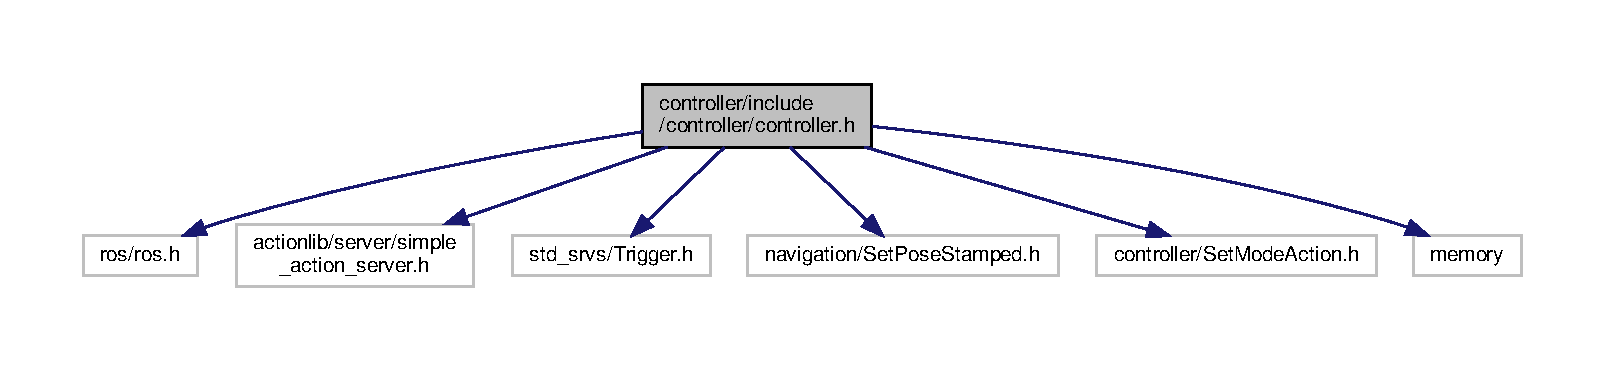
\includegraphics[width=350pt]{controller_8h__incl}
\end{center}
\end{figure}
This graph shows which files directly or indirectly include this file\+:
\nopagebreak
\begin{figure}[H]
\begin{center}
\leavevmode
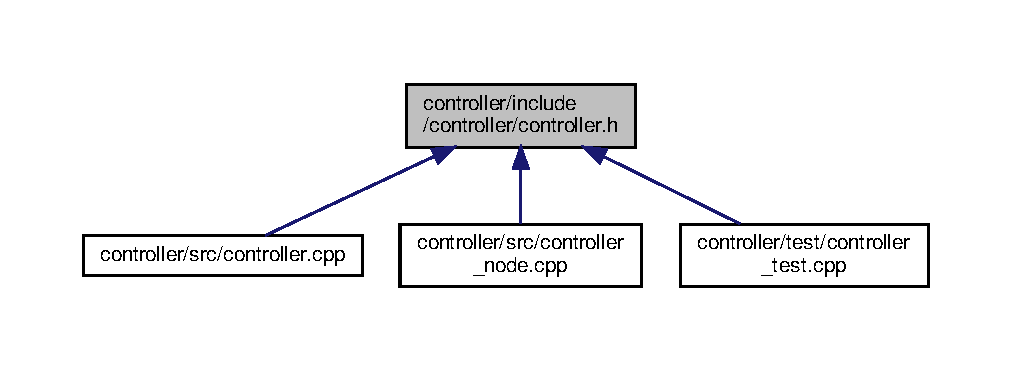
\includegraphics[width=350pt]{controller_8h__dep__incl}
\end{center}
\end{figure}
\subsection*{Classes}
\begin{DoxyCompactItemize}
\item 
class \hyperlink{classcleanup_1_1_controller}{cleanup\+::\+Controller}
\begin{DoxyCompactList}\small\item\em Implementation for a \hyperlink{classcleanup_1_1_controller}{Controller} in R\+OS to command a turtlebot rover. \end{DoxyCompactList}\end{DoxyCompactItemize}
\subsection*{Namespaces}
\begin{DoxyCompactItemize}
\item 
 \hyperlink{namespacecleanup}{cleanup}
\begin{DoxyCompactList}\small\item\em Namespace for Cleanup Implementation. \end{DoxyCompactList}\end{DoxyCompactItemize}


\subsection{Detailed Description}
Header of the Controller class for overall system management. 

\begin{DoxyCopyright}{Copyright}
\mbox{[}2020\mbox{]} $<$Daniel Sahu, Spencer Elyard, Santosh Kesani$>$ 
\end{DoxyCopyright}

\hypertarget{controller_8cpp}{}\section{controller/src/controller.cpp File Reference}
\label{controller_8cpp}\index{controller/src/controller.\+cpp@{controller/src/controller.\+cpp}}


Implementation of the Controller class for overall system management.  


{\ttfamily \#include $<$controller/controller.\+h$>$}\newline
{\ttfamily \#include $<$actionlib/server/simple\+\_\+action\+\_\+server.\+h$>$}\newline
Include dependency graph for controller.\+cpp\+:\nopagebreak
\begin{figure}[H]
\begin{center}
\leavevmode
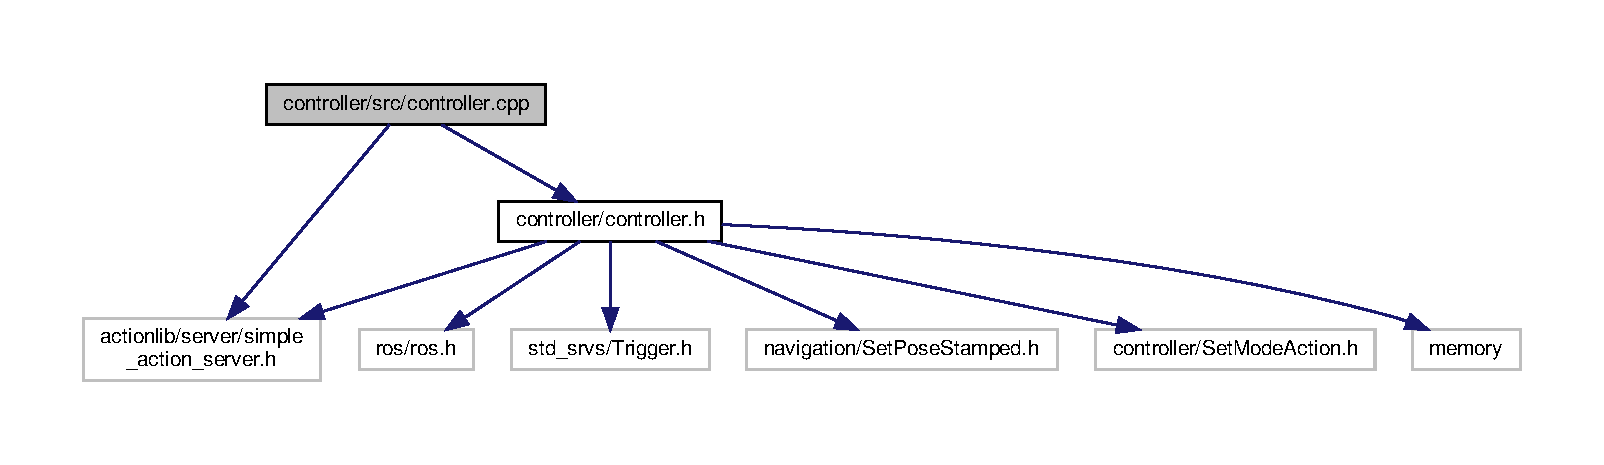
\includegraphics[width=350pt]{controller_8cpp__incl}
\end{center}
\end{figure}
\subsection*{Namespaces}
\begin{DoxyCompactItemize}
\item 
 \hyperlink{namespacecleanup}{cleanup}
\begin{DoxyCompactList}\small\item\em Namespace for Cleanup Implementation. \end{DoxyCompactList}\end{DoxyCompactItemize}


\subsection{Detailed Description}
Implementation of the Controller class for overall system management. 

\begin{DoxyCopyright}{Copyright}
\mbox{[}2020\mbox{]} $<$Daniel Sahu, Spencer Elyard, Santosh Kesani$>$ 
\end{DoxyCopyright}

\hypertarget{controller__node_8cpp}{}\section{controller/src/controller\+\_\+node.cpp File Reference}
\label{controller__node_8cpp}\index{controller/src/controller\+\_\+node.\+cpp@{controller/src/controller\+\_\+node.\+cpp}}


Instantiation of the Controller class for overall system management.  


{\ttfamily \#include $<$ros/ros.\+h$>$}\newline
{\ttfamily \#include $<$controller/controller.\+h$>$}\newline
Include dependency graph for controller\+\_\+node.\+cpp\+:
\nopagebreak
\begin{figure}[H]
\begin{center}
\leavevmode
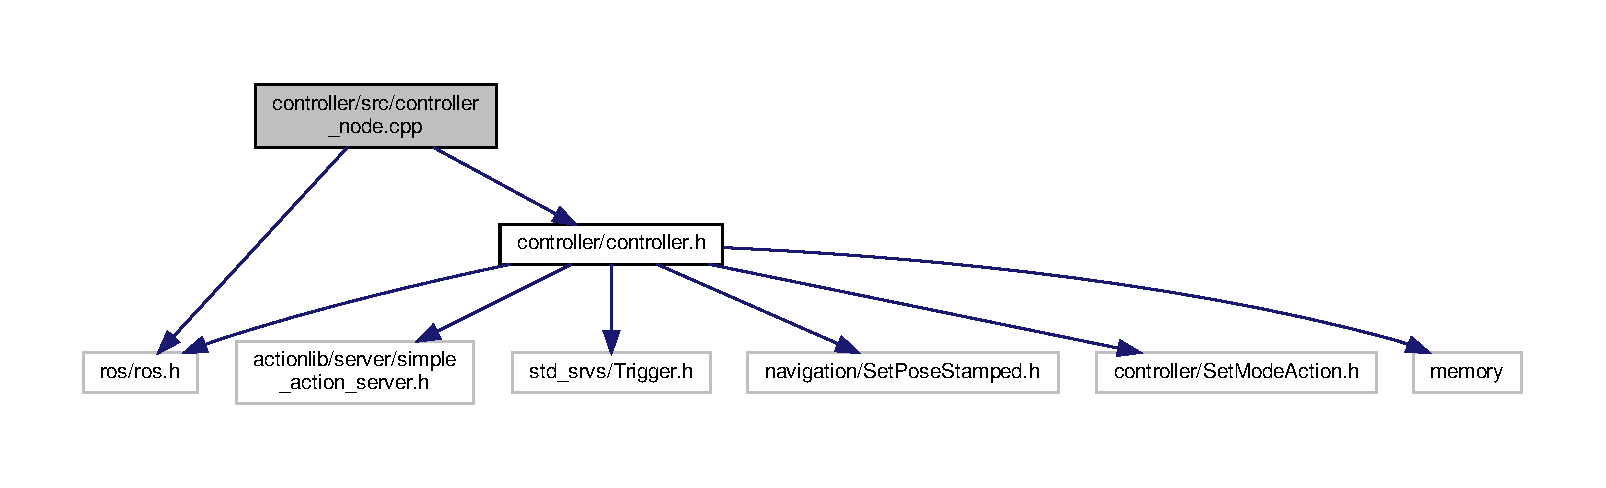
\includegraphics[width=350pt]{controller__node_8cpp__incl}
\end{center}
\end{figure}
\subsection*{Functions}
\begin{DoxyCompactItemize}
\item 
\mbox{\Hypertarget{controller__node_8cpp_a3c04138a5bfe5d72780bb7e82a18e627}\label{controller__node_8cpp_a3c04138a5bfe5d72780bb7e82a18e627}} 
int {\bfseries main} (int argc, char $\ast$$\ast$argv)
\end{DoxyCompactItemize}


\subsection{Detailed Description}
Instantiation of the Controller class for overall system management. 

\begin{DoxyCopyright}{Copyright}
\mbox{[}2020\mbox{]} $<$Daniel Sahu, Spencer Elyard, Santosh Kesani$>$ 
\end{DoxyCopyright}

\hypertarget{user__panel_8cpp}{}\section{controller/src/user\+\_\+panel.cpp File Reference}
\label{user__panel_8cpp}\index{controller/src/user\+\_\+panel.\+cpp@{controller/src/user\+\_\+panel.\+cpp}}


Implementation of custom R\+V\+IZ user panel for control.  


{\ttfamily \#include \char`\"{}user\+\_\+panel.\+h\char`\"{}}\newline
{\ttfamily \#include $<$stdio.\+h$>$}\newline
{\ttfamily \#include $<$geometry\+\_\+msgs/\+Twist.\+h$>$}\newline
{\ttfamily \#include $<$pluginlib/class\+\_\+list\+\_\+macros.\+h$>$}\newline
{\ttfamily \#include $<$Q\+Painter$>$}\newline
{\ttfamily \#include $<$Q\+Line\+Edit$>$}\newline
{\ttfamily \#include $<$Q\+V\+Box\+Layout$>$}\newline
{\ttfamily \#include $<$Q\+H\+Box\+Layout$>$}\newline
{\ttfamily \#include $<$Q\+Label$>$}\newline
{\ttfamily \#include $<$Q\+Timer$>$}\newline
{\ttfamily \#include $<$Q\+Push\+Button$>$}\newline
{\ttfamily \#include $<$string$>$}\newline
Include dependency graph for user\+\_\+panel.\+cpp\+:
\nopagebreak
\begin{figure}[H]
\begin{center}
\leavevmode
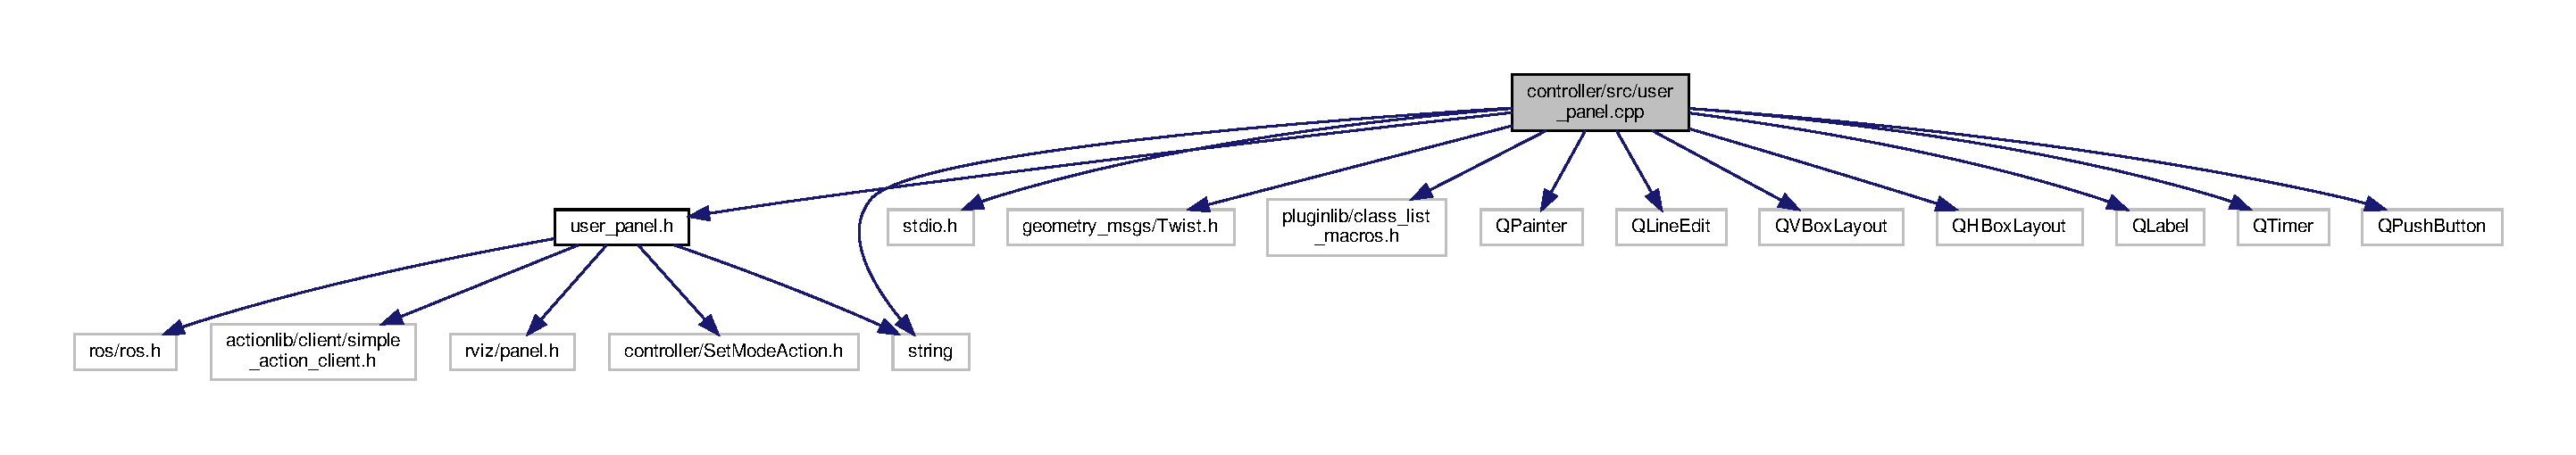
\includegraphics[width=350pt]{user__panel_8cpp__incl}
\end{center}
\end{figure}
\subsection*{Namespaces}
\begin{DoxyCompactItemize}
\item 
 \hyperlink{namespacecleanup}{cleanup}
\begin{DoxyCompactList}\small\item\em Namespace for Cleanup Implementation. \end{DoxyCompactList}\end{DoxyCompactItemize}


\subsection{Detailed Description}
Implementation of custom R\+V\+IZ user panel for control. 

\begin{DoxyCopyright}{Copyright}
\mbox{[}2020\mbox{]} $<$Daniel Sahu, Spencer Elyard, Santosh Kesani$>$ 
\end{DoxyCopyright}

\hypertarget{user__panel_8h}{}\section{controller/src/user\+\_\+panel.h File Reference}
\label{user__panel_8h}\index{controller/src/user\+\_\+panel.\+h@{controller/src/user\+\_\+panel.\+h}}


Implementation of custom R\+V\+IZ user panel for control.  


{\ttfamily \#include $<$ros/ros.\+h$>$}\newline
{\ttfamily \#include $<$actionlib/client/simple\+\_\+action\+\_\+client.\+h$>$}\newline
{\ttfamily \#include $<$rviz/panel.\+h$>$}\newline
{\ttfamily \#include $<$controller/\+Set\+Mode\+Action.\+h$>$}\newline
{\ttfamily \#include $<$string$>$}\newline
Include dependency graph for user\+\_\+panel.\+h\+:\nopagebreak
\begin{figure}[H]
\begin{center}
\leavevmode
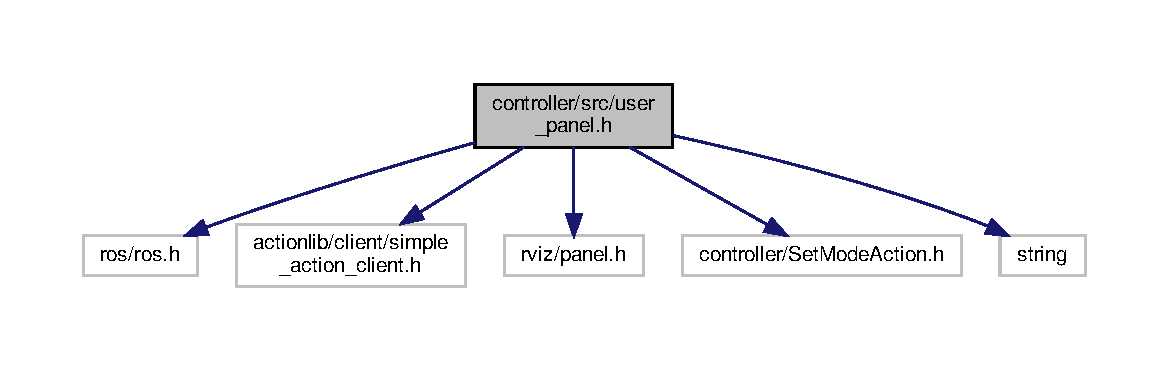
\includegraphics[width=350pt]{user__panel_8h__incl}
\end{center}
\end{figure}
This graph shows which files directly or indirectly include this file\+:\nopagebreak
\begin{figure}[H]
\begin{center}
\leavevmode
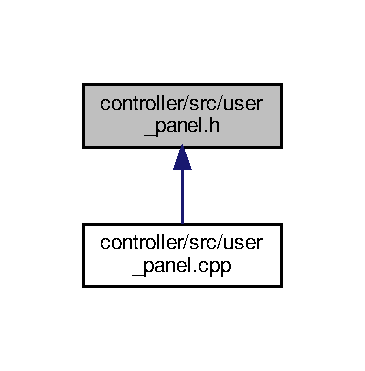
\includegraphics[width=175pt]{user__panel_8h__dep__incl}
\end{center}
\end{figure}
\subsection*{Classes}
\begin{DoxyCompactItemize}
\item 
class \hyperlink{classcleanup_1_1_user_panel}{cleanup\+::\+User\+Panel}
\begin{DoxyCompactList}\small\item\em Implementation for a custom user panel in R\+V\+IZ. \end{DoxyCompactList}\end{DoxyCompactItemize}
\subsection*{Namespaces}
\begin{DoxyCompactItemize}
\item 
 \hyperlink{namespacecleanup}{cleanup}
\begin{DoxyCompactList}\small\item\em Namespace for Cleanup Implementation. \end{DoxyCompactList}\end{DoxyCompactItemize}


\subsection{Detailed Description}
Implementation of custom R\+V\+IZ user panel for control. 

\begin{DoxyCopyright}{Copyright}
\mbox{[}2020\mbox{]} $<$Daniel Sahu, Spencer Elyard, Santosh Kesani$>$ 
\end{DoxyCopyright}

\hypertarget{controller__test_8cpp}{}\section{controller/test/controller\+\_\+test.cpp File Reference}
\label{controller__test_8cpp}\index{controller/test/controller\+\_\+test.\+cpp@{controller/test/controller\+\_\+test.\+cpp}}


Implementation of the Controller test.  


{\ttfamily \#include $<$ros/ros.\+h$>$}\newline
{\ttfamily \#include $<$controller/controller.\+h$>$}\newline
{\ttfamily \#include $<$gtest/gtest.\+h$>$}\newline
{\ttfamily \#include $<$controller/\+Set\+Mode\+Action.\+h$>$}\newline
{\ttfamily \#include $<$actionlib/client/simple\+\_\+action\+\_\+client.\+h$>$}\newline
{\ttfamily \#include $<$thread$>$}\newline
Include dependency graph for controller\+\_\+test.\+cpp\+:
\nopagebreak
\begin{figure}[H]
\begin{center}
\leavevmode
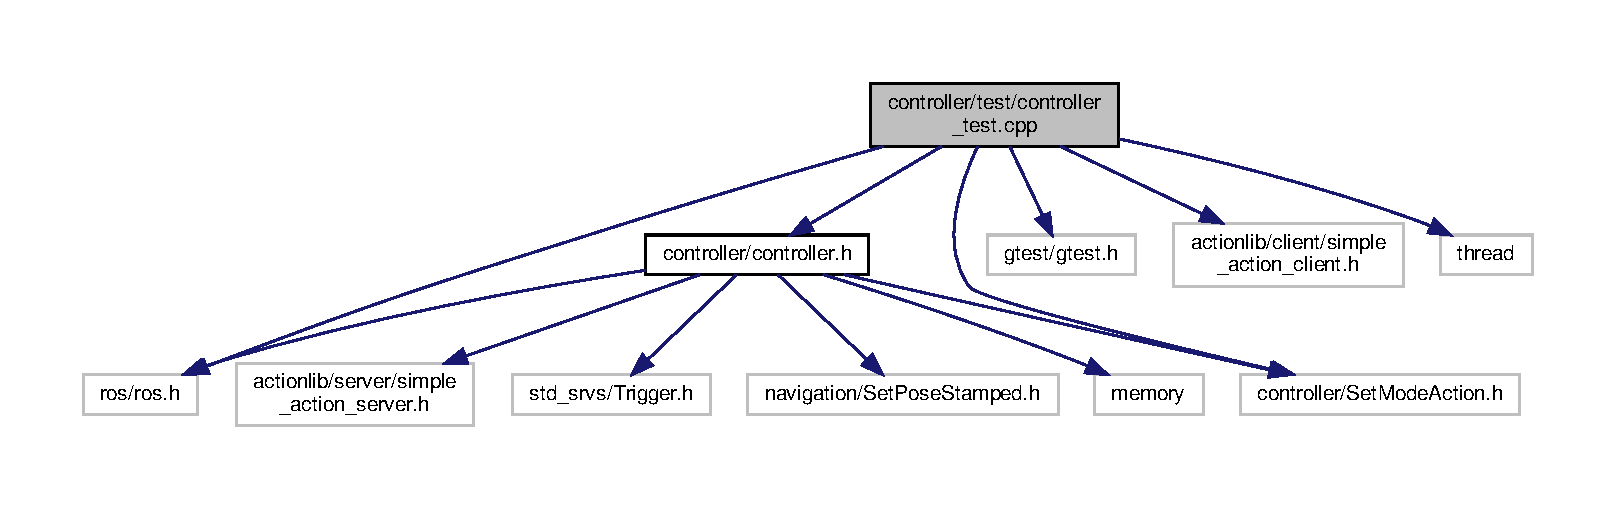
\includegraphics[width=350pt]{controller__test_8cpp__incl}
\end{center}
\end{figure}
\subsection*{Functions}
\begin{DoxyCompactItemize}
\item 
\mbox{\Hypertarget{controller__test_8cpp_a5df6b5c1f9569aeae5a5a61aa79235c1}\label{controller__test_8cpp_a5df6b5c1f9569aeae5a5a61aa79235c1}} 
{\bfseries T\+E\+ST} (Controller\+\_\+\+Test\+Services\+Exist, should\+\_\+pass)
\item 
\mbox{\Hypertarget{controller__test_8cpp_a35e9425ef4ff8ca09af4d66c9e7e839d}\label{controller__test_8cpp_a35e9425ef4ff8ca09af4d66c9e7e839d}} 
{\bfseries T\+E\+ST} (Controller\+\_\+\+Test\+Action\+Client\+\_\+\+Bad\+Goal, should\+\_\+fail)
\item 
\mbox{\Hypertarget{controller__test_8cpp_a58b52bfdec32a14cfa9315be9d70bf3b}\label{controller__test_8cpp_a58b52bfdec32a14cfa9315be9d70bf3b}} 
{\bfseries T\+E\+ST} (Controller\+\_\+\+Test\+Execute\+\_\+\+Clean\+Goal, should\+\_\+pass)
\item 
\mbox{\Hypertarget{controller__test_8cpp_aa92425a61876bc963bb7c2edaafd691c}\label{controller__test_8cpp_aa92425a61876bc963bb7c2edaafd691c}} 
{\bfseries T\+E\+ST} (Controller\+\_\+\+Test\+Execute\+\_\+\+Explore\+Goal, should\+\_\+pass)
\item 
\mbox{\Hypertarget{controller__test_8cpp_a3c04138a5bfe5d72780bb7e82a18e627}\label{controller__test_8cpp_a3c04138a5bfe5d72780bb7e82a18e627}} 
int {\bfseries main} (int argc, char $\ast$$\ast$argv)
\end{DoxyCompactItemize}
\subsection*{Variables}
\begin{DoxyCompactItemize}
\item 
\mbox{\Hypertarget{controller__test_8cpp_a5100c270de053238ccc5696857cec6f3}\label{controller__test_8cpp_a5100c270de053238ccc5696857cec6f3}} 
std\+::unique\+\_\+ptr$<$ \hyperlink{classcleanup_1_1_controller}{cleanup\+::\+Controller} $>$ {\bfseries ctrl}
\item 
\mbox{\Hypertarget{controller__test_8cpp_a7d6d3de9ddf4963eb3ea112920944a87}\label{controller__test_8cpp_a7d6d3de9ddf4963eb3ea112920944a87}} 
std\+::shared\+\_\+ptr$<$ ros\+::\+Node\+Handle $>$ {\bfseries nh}
\end{DoxyCompactItemize}


\subsection{Detailed Description}
Implementation of the Controller test. 

\begin{DoxyCopyright}{Copyright}
\mbox{[}2020\mbox{]} $<$Daniel Sahu, Spencer Elyard, Santosh Kesani$>$ 
\end{DoxyCopyright}

\hypertarget{navigation_8h}{}\section{navigation/include/navigation/navigation.h File Reference}
\label{navigation_8h}\index{navigation/include/navigation/navigation.\+h@{navigation/include/navigation/navigation.\+h}}


Header of the Navigation class for basic navigation.  


{\ttfamily \#include $<$ros/ros.\+h$>$}\newline
{\ttfamily \#include $<$tf2/\+Linear\+Math/\+Transform.\+h$>$}\newline
{\ttfamily \#include $<$tf2\+\_\+ros/transform\+\_\+listener.\+h$>$}\newline
{\ttfamily \#include $<$tf2\+\_\+ros/buffer.\+h$>$}\newline
{\ttfamily \#include $<$tf2\+\_\+geometry\+\_\+msgs/tf2\+\_\+geometry\+\_\+msgs.\+h$>$}\newline
{\ttfamily \#include $<$actionlib/client/simple\+\_\+action\+\_\+client.\+h$>$}\newline
{\ttfamily \#include $<$move\+\_\+base\+\_\+msgs/\+Move\+Base\+Action.\+h$>$}\newline
{\ttfamily \#include $<$geometry\+\_\+msgs/\+Pose\+Stamped.\+h$>$}\newline
{\ttfamily \#include $<$std\+\_\+srvs/\+Trigger.\+h$>$}\newline
{\ttfamily \#include $<$navigation/\+Set\+Pose\+Stamped.\+h$>$}\newline
{\ttfamily \#include $<$atomic$>$}\newline
{\ttfamily \#include $<$future$>$}\newline
{\ttfamily \#include $<$memory$>$}\newline
{\ttfamily \#include $<$string$>$}\newline
Include dependency graph for navigation.\+h\+:
\nopagebreak
\begin{figure}[H]
\begin{center}
\leavevmode
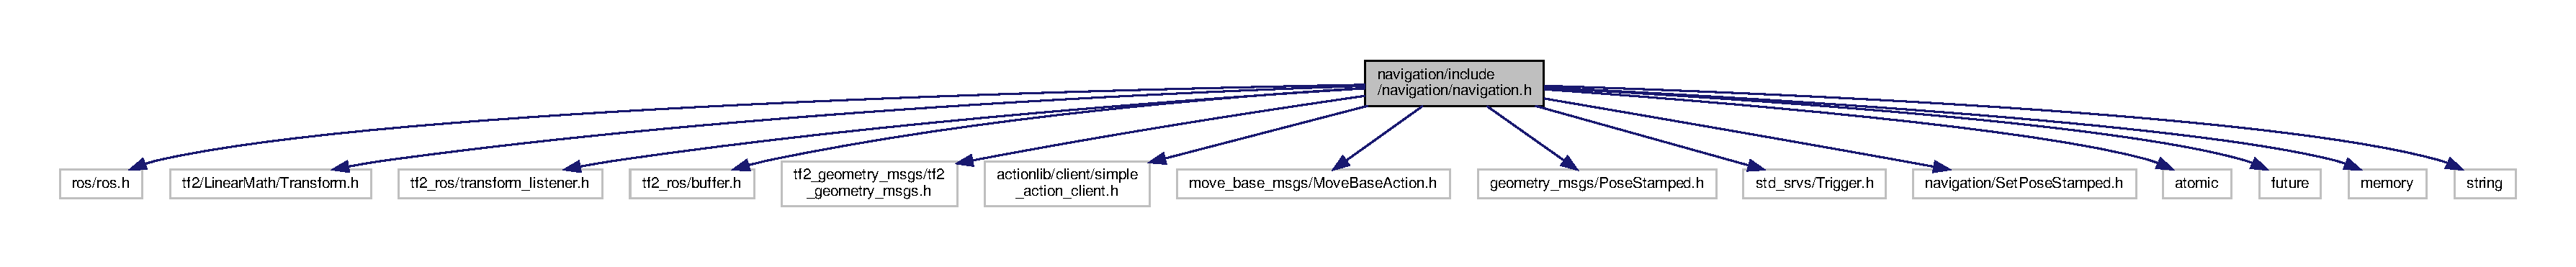
\includegraphics[width=350pt]{navigation_8h__incl}
\end{center}
\end{figure}
This graph shows which files directly or indirectly include this file\+:
\nopagebreak
\begin{figure}[H]
\begin{center}
\leavevmode
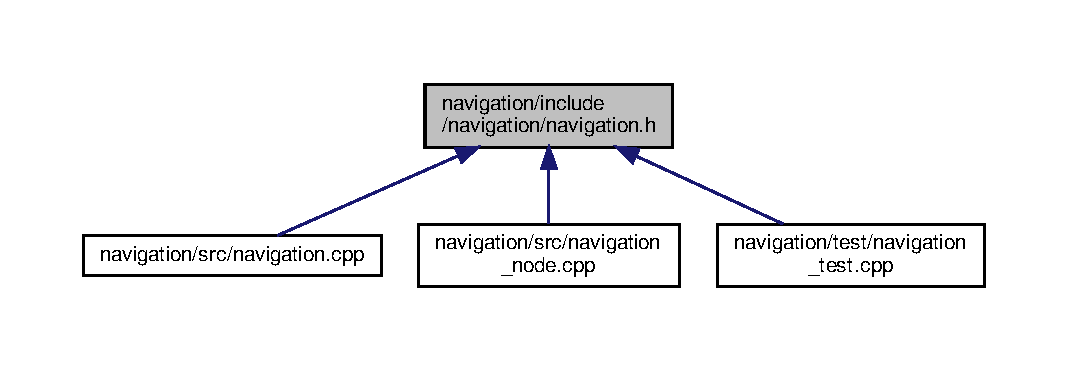
\includegraphics[width=350pt]{navigation_8h__dep__incl}
\end{center}
\end{figure}
\subsection*{Classes}
\begin{DoxyCompactItemize}
\item 
class \hyperlink{classcleanup_1_1_navigation}{cleanup\+::\+Navigation}
\begin{DoxyCompactList}\small\item\em Implementation for navigation routines in R\+OS to command a turtlebot rover. \end{DoxyCompactList}\end{DoxyCompactItemize}
\subsection*{Namespaces}
\begin{DoxyCompactItemize}
\item 
 \hyperlink{namespacecleanup}{cleanup}
\begin{DoxyCompactList}\small\item\em Namespace for Cleanup Implementation. \end{DoxyCompactList}\end{DoxyCompactItemize}


\subsection{Detailed Description}
Header of the Navigation class for basic navigation. 

\begin{DoxyCopyright}{Copyright}
\mbox{[}2020\mbox{]} $<$Daniel Sahu, Spencer Elyard, Santosh Kesani$>$ 
\end{DoxyCopyright}

\hypertarget{navigation_8cpp}{}\section{navigation/src/navigation.cpp File Reference}
\label{navigation_8cpp}\index{navigation/src/navigation.\+cpp@{navigation/src/navigation.\+cpp}}


Implementation of the Navigation class for basic navigation.  


{\ttfamily \#include $<$navigation/navigation.\+h$>$}\newline
Include dependency graph for navigation.\+cpp\+:
\nopagebreak
\begin{figure}[H]
\begin{center}
\leavevmode
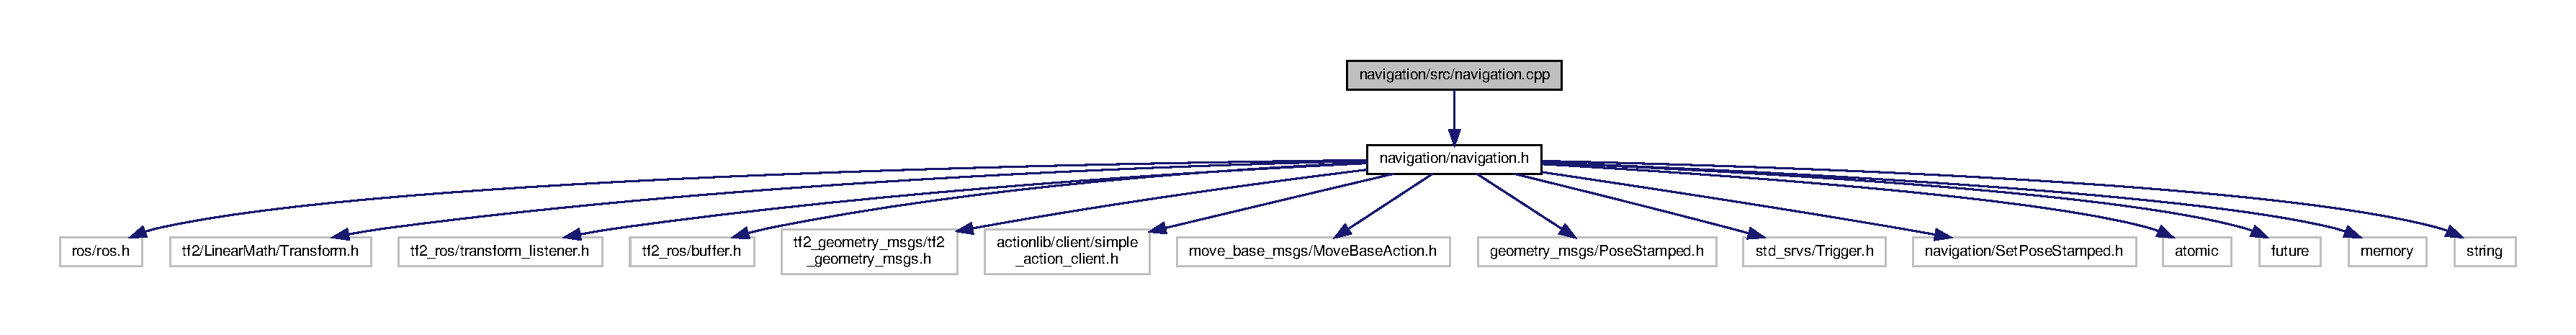
\includegraphics[width=350pt]{navigation_8cpp__incl}
\end{center}
\end{figure}
\subsection*{Namespaces}
\begin{DoxyCompactItemize}
\item 
 \hyperlink{namespacecleanup}{cleanup}
\begin{DoxyCompactList}\small\item\em Namespace for Cleanup Implementation. \end{DoxyCompactList}\end{DoxyCompactItemize}


\subsection{Detailed Description}
Implementation of the Navigation class for basic navigation. 

\begin{DoxyCopyright}{Copyright}
\mbox{[}2020\mbox{]} $<$Daniel Sahu, Spencer Elyard, Santosh Kesani$>$ 
\end{DoxyCopyright}

\hypertarget{navigation__node_8cpp}{}\section{navigation/src/navigation\+\_\+node.cpp File Reference}
\label{navigation__node_8cpp}\index{navigation/src/navigation\+\_\+node.\+cpp@{navigation/src/navigation\+\_\+node.\+cpp}}


R\+OS Node instantiation fo Navigation.  


{\ttfamily \#include $<$ros/ros.\+h$>$}\newline
{\ttfamily \#include $<$navigation/navigation.\+h$>$}\newline
Include dependency graph for navigation\+\_\+node.\+cpp\+:
\nopagebreak
\begin{figure}[H]
\begin{center}
\leavevmode
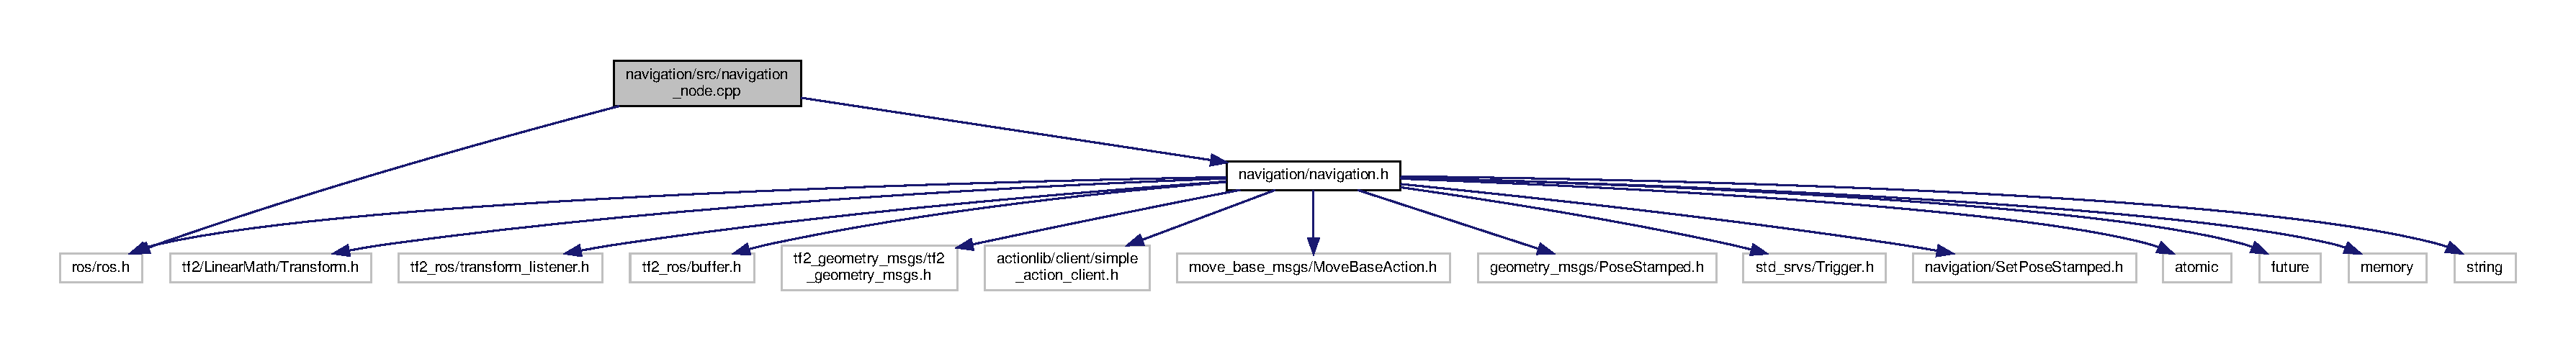
\includegraphics[width=350pt]{navigation__node_8cpp__incl}
\end{center}
\end{figure}
\subsection*{Functions}
\begin{DoxyCompactItemize}
\item 
\mbox{\Hypertarget{navigation__node_8cpp_a3c04138a5bfe5d72780bb7e82a18e627}\label{navigation__node_8cpp_a3c04138a5bfe5d72780bb7e82a18e627}} 
int {\bfseries main} (int argc, char $\ast$$\ast$argv)
\end{DoxyCompactItemize}


\subsection{Detailed Description}
R\+OS Node instantiation fo Navigation. 

\begin{DoxyCopyright}{Copyright}
\mbox{[}2020\mbox{]} $<$Daniel Sahu, Spencer Elyard, Santosh Kesani$>$ 
\end{DoxyCopyright}

\hypertarget{navigation__test_8cpp}{}\section{navigation/test/navigation\+\_\+test.cpp File Reference}
\label{navigation__test_8cpp}\index{navigation/test/navigation\+\_\+test.\+cpp@{navigation/test/navigation\+\_\+test.\+cpp}}


Implementation of the Navigation test.  


{\ttfamily \#include $<$ros/ros.\+h$>$}\newline
{\ttfamily \#include $<$ros/service\+\_\+client.\+h$>$}\newline
{\ttfamily \#include $<$navigation/navigation.\+h$>$}\newline
{\ttfamily \#include $<$gtest/gtest.\+h$>$}\newline
{\ttfamily \#include $<$std\+\_\+srvs/\+Trigger.\+h$>$}\newline
{\ttfamily \#include $<$navigation/\+Set\+Pose\+Stamped.\+h$>$}\newline
{\ttfamily \#include $<$move\+\_\+base\+\_\+msgs/\+Move\+Base\+Action.\+h$>$}\newline
{\ttfamily \#include $<$cmath$>$}\newline
{\ttfamily \#include $<$thread$>$}\newline
Include dependency graph for navigation\+\_\+test.\+cpp\+:\nopagebreak
\begin{figure}[H]
\begin{center}
\leavevmode
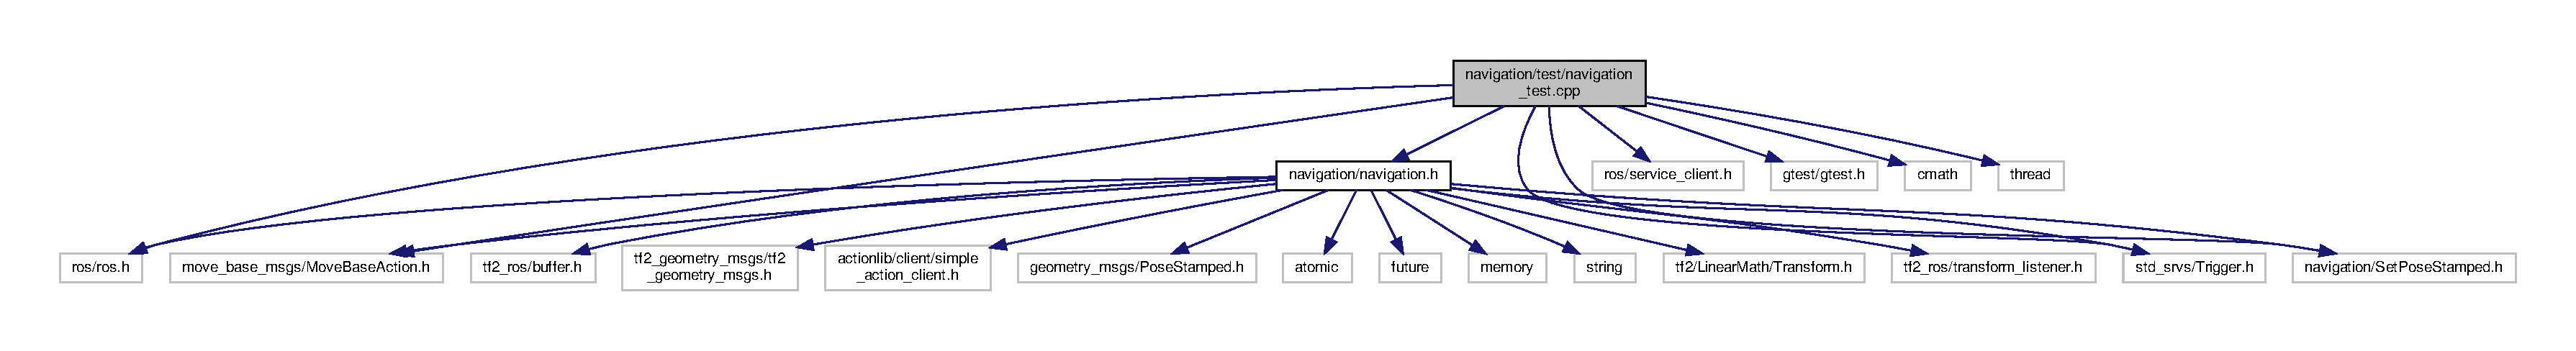
\includegraphics[width=350pt]{navigation__test_8cpp__incl}
\end{center}
\end{figure}
\subsection*{Functions}
\begin{DoxyCompactItemize}
\item 
\mbox{\Hypertarget{navigation__test_8cpp_a467037c72fb6b412a518c596fde1680e}\label{navigation__test_8cpp_a467037c72fb6b412a518c596fde1680e}} 
\hyperlink{navigation__test_8cpp_a467037c72fb6b412a518c596fde1680e}{T\+E\+ST} (Navigation\+\_\+\+Test, get\+Nav\+Mode\+Default)
\begin{DoxyCompactList}\small\item\em Check to ensure able to get current nav mode (default = 0) \end{DoxyCompactList}\item 
\mbox{\Hypertarget{navigation__test_8cpp_a9404d72b3f2daeb180a6828166fa1a13}\label{navigation__test_8cpp_a9404d72b3f2daeb180a6828166fa1a13}} 
\hyperlink{navigation__test_8cpp_a9404d72b3f2daeb180a6828166fa1a13}{T\+E\+ST} (Navigation\+\_\+\+Test, Get\+Pose)
\begin{DoxyCompactList}\small\item\em Check to ensure the get\+Robot\+Pose() command works with the launch values Note Z height difference from robot config file. \end{DoxyCompactList}\item 
\mbox{\Hypertarget{navigation__test_8cpp_a85c9218cda8800a6d8022116611c7153}\label{navigation__test_8cpp_a85c9218cda8800a6d8022116611c7153}} 
\hyperlink{navigation__test_8cpp_a85c9218cda8800a6d8022116611c7153}{T\+E\+ST} (Navigation\+\_\+\+Test, stop\+Service\+Starts)
\begin{DoxyCompactList}\small\item\em Check to ensure the \char`\"{}\+Stop\char`\"{} service starts and triggers correct nav mode. \end{DoxyCompactList}\item 
\mbox{\Hypertarget{navigation__test_8cpp_a08cf090894a2ea5461dec4f093a3fa13}\label{navigation__test_8cpp_a08cf090894a2ea5461dec4f093a3fa13}} 
\hyperlink{navigation__test_8cpp_a08cf090894a2ea5461dec4f093a3fa13}{T\+E\+ST} (Navigation\+\_\+\+Test, explore\+Service\+Starts)
\begin{DoxyCompactList}\small\item\em Check to ensure the \char`\"{}\+Explore\char`\"{} service starts and triggers correct nav mode. \end{DoxyCompactList}\item 
\mbox{\Hypertarget{navigation__test_8cpp_a2477ea0f0f5cb5e91764dd888d03f5c7}\label{navigation__test_8cpp_a2477ea0f0f5cb5e91764dd888d03f5c7}} 
\hyperlink{navigation__test_8cpp_a2477ea0f0f5cb5e91764dd888d03f5c7}{T\+E\+ST} (Navigation\+\_\+\+Test, goto\+Service\+Starts)
\begin{DoxyCompactList}\small\item\em Check to ensure the \char`\"{}\+Go\+To\char`\"{} service starts and triggers correct nav mode. \end{DoxyCompactList}\item 
\mbox{\Hypertarget{navigation__test_8cpp_a52f0baf04248458a54fdc41c4c1c4977}\label{navigation__test_8cpp_a52f0baf04248458a54fdc41c4c1c4977}} 
\hyperlink{navigation__test_8cpp_a52f0baf04248458a54fdc41c4c1c4977}{T\+E\+ST} (Navigation\+\_\+\+Test, explore\+Loop)
\begin{DoxyCompactList}\small\item\em Check to ensure the \char`\"{}\+Explore Loop\char`\"{} starts correctly. \end{DoxyCompactList}\item 
\mbox{\Hypertarget{navigation__test_8cpp_ae02285d0ca4206028fdfd3a632047caa}\label{navigation__test_8cpp_ae02285d0ca4206028fdfd3a632047caa}} 
\hyperlink{navigation__test_8cpp_ae02285d0ca4206028fdfd3a632047caa}{T\+E\+ST} (Navigation\+\_\+\+Test, stop\+Command)
\begin{DoxyCompactList}\small\item\em Check to ensure the \char`\"{}\+Stop\char`\"{} function calls correctly. \end{DoxyCompactList}\item 
\mbox{\Hypertarget{navigation__test_8cpp_a3c04138a5bfe5d72780bb7e82a18e627}\label{navigation__test_8cpp_a3c04138a5bfe5d72780bb7e82a18e627}} 
int \hyperlink{navigation__test_8cpp_a3c04138a5bfe5d72780bb7e82a18e627}{main} (int argc, char $\ast$$\ast$argv)
\begin{DoxyCompactList}\small\item\em Main loop. \end{DoxyCompactList}\end{DoxyCompactItemize}
\subsection*{Variables}
\begin{DoxyCompactItemize}
\item 
\mbox{\Hypertarget{navigation__test_8cpp_a75205abae44efc7d1f0da03b3650a45a}\label{navigation__test_8cpp_a75205abae44efc7d1f0da03b3650a45a}} 
std\+::unique\+\_\+ptr$<$ \hyperlink{classcleanup_1_1_navigation}{cleanup\+::\+Navigation} $>$ {\bfseries nav}
\item 
\mbox{\Hypertarget{navigation__test_8cpp_a7d6d3de9ddf4963eb3ea112920944a87}\label{navigation__test_8cpp_a7d6d3de9ddf4963eb3ea112920944a87}} 
std\+::shared\+\_\+ptr$<$ ros\+::\+Node\+Handle $>$ {\bfseries nh}
\end{DoxyCompactItemize}


\subsection{Detailed Description}
Implementation of the Navigation test. 

\begin{DoxyCopyright}{Copyright}
\mbox{[}2020\mbox{]} $<$Daniel Sahu, Spencer Elyard, Santosh Kesani$>$ 
\end{DoxyCopyright}

%--- End generated contents ---

% Index
\backmatter
\newpage
\phantomsection
\clearemptydoublepage
\addcontentsline{toc}{chapter}{Index}
\printindex

\end{document}
